\documentclass[a4paper]{article}

\usepackage{hyperref}
\usepackage{graphicx}
\usepackage{caption}
\usepackage{subcaption}
\usepackage{kpfonts}
\graphicspath{ {img/} }

\usepackage{amsmath}
\usepackage{bbm}
\usepackage{dsfont}
\usepackage{amsfonts}
\usepackage{amsthm}
\usepackage{mathtools}
\usepackage{gensymb}
\usepackage[margin=1in]{geometry}
\usepackage{tabto}
\usepackage{xcolor}

\geometry{rmargin=1.5in}

\makeatletter
% \renewcommand\section{\@startsection{section}{1}{\z@}%
%                                   {-3.5ex \@plus -1ex \@minus -.2ex}%
%                                   {2.3ex \@plus.2ex}%
%                                   {\normalfont\normalsize\bfseries}}
\makeatletter


\title{\Large Estimation of Laplace Series Coefficients via 2-D Numerical Quadrature}
\author{Evan Voyles}
\date{}

\newtheorem{theorem}{Th\'eor\`eme}
\newtheorem*{theorem*}{Th\'eor\`eme}
\newtheorem{exercice}{Exercice}
\newtheorem*{exercice*}{Exercice bonus}
\theoremstyle{definition}
\newtheorem{definition}{D\'efinition}
\newtheorem*{definition*}{D\'efinition}
\newtheorem{lemme}{Lemme}
\newtheorem{proposition}{Proposition}
\newtheorem*{proposition*}{Proposition}

\begin{document}

\makeatletter
\maketitle
\begin{center}
    \vspace{-.2in}
    \today
\end{center}
\makeatother

\newenvironment{norm}{
    \normalfont
}


\section{Abstract}

This paper provides an alternative approach to the computation
of Laplace Series coefficients $C_l^m$ and $S_l^m$ with algorithmic complexity $O(Nl^2)$ in time and $O(Nl^2)$ in space. We 
make use of the fact that the spherical harmonics form a complete and orthogonal set to directly
compute $C_l^m$ as a 2-dimensional integral. We estimate this integral using numerical quadrature techniques
and the resulting model is blazing fast compared to a least squares model running in $O(Nl^4$). Harnessing the structure of the 
data sets, we perform many optimization to reduce the amount of data needed to be stored in memory and save time by precomputing values of the 
associated Legendre polynomials. We explore the scalability of this algorithm when implemented in parallel and we present a high-degree model of the
ultra data set.



\section{Preliminaries}

Any sufficiently regular function defined on a sphere can be written
\begin{equation} \label{eq:f_iso}
    f(\theta, \phi) = \sum_{l = 0}^{+\infty}\sum_{m = 0}^l \bar P_l^m(\cos\theta)[C_l^m\cos m\phi + S_l^m \sin m \phi].
\end{equation}

Where $C_l^m, S_l^m$ are \textit{spherical harmonic} coefficients (also referred to as Laplace series coefficients) of 
degree \textit{l} and order \textit{m}; $\bar P_l^m$ are the fully normalized Associated Legendre Functions of degree $l$ and order $m$;
$\theta$ is the polar angle and $\phi$ is the azimuthal angle, as per ISO convention\footnote{We have chosen the ISO standard coordinate system to 
ensure the integrity of future computations. For a discussion on transforming the $(\phi, \lambda)$ coordinates provided by NASA, see Appendix A}.

The project proposal suggests computing the coefficients $C_l^m, S_l^m$ by setting up an overdetermined linear system of equations and finding the least squares
solution. Unfortunately, this problem runs in $O(Nl_{max}^4)$ time and requires about $8N(l_{max} + 1)^2$ bytes of memory. That is absurdly prohibitive. Furthermore, there 
are no \textit{self-evident} parallelization techniques to speed up computation time. In this report we propose an alternative approach to computing the Laplace series coefficients
$C_l^m$ and $S_l^m$ that runs in \textbf{$O(Nl^2)$} time complexity with trivial parallelization models.

\subsection{Laplace Series Coefficients}

The coefficients $C_l^m$ and $S_l^m$ are defined as the orthogonal projection of $f(\theta, \phi)$ onto the basis functions $Y_l^m$, 
the spherical harmonics of degree $l$ and order $m$. This definition is perfectly analagous to the fourier coefficients for $2\pi$ 
periodic functions. Written in terms of the normalized legendre polynomials, these projections are defined as:

\begin{align*}
    \label{eq:coeff}
    C_l^m &= \int_0^{2\pi}\int_0^\pi f(\theta, \phi) \bar P_l^m (\cos \theta)\cos (m \phi) \sin \theta d\theta d\phi\\
    S_l^m &= \int_0^{2\pi}\int_0^\pi f(\theta, \phi) \bar P_l^m (\cos \theta)\sin (m \phi) \sin \theta d\theta d\phi 
\end{align*}

We propose a solution to directly compute an approximation of the $C_l^m$ and $S_l^m$ using numerical integration.

\newpage

\section{Data Sets}

NASA data sets contain the altitude information for a spherical coordinate pair. The spherical coordinates can
be represented as the discretization of a 2-d rectangle with width $2\pi$ and height $\pi$. NASA's data sets contain observations
over a discretization of $[-\frac{\pi}{2}, \frac{\pi}{2}] \times [-\pi, \pi]$, represented as a $n_\theta \times n_\phi$ grid with equidistant points.

\begin{figure}[h!]
    \centering
    \begin{minipage}{.5\textwidth}
      \centering
      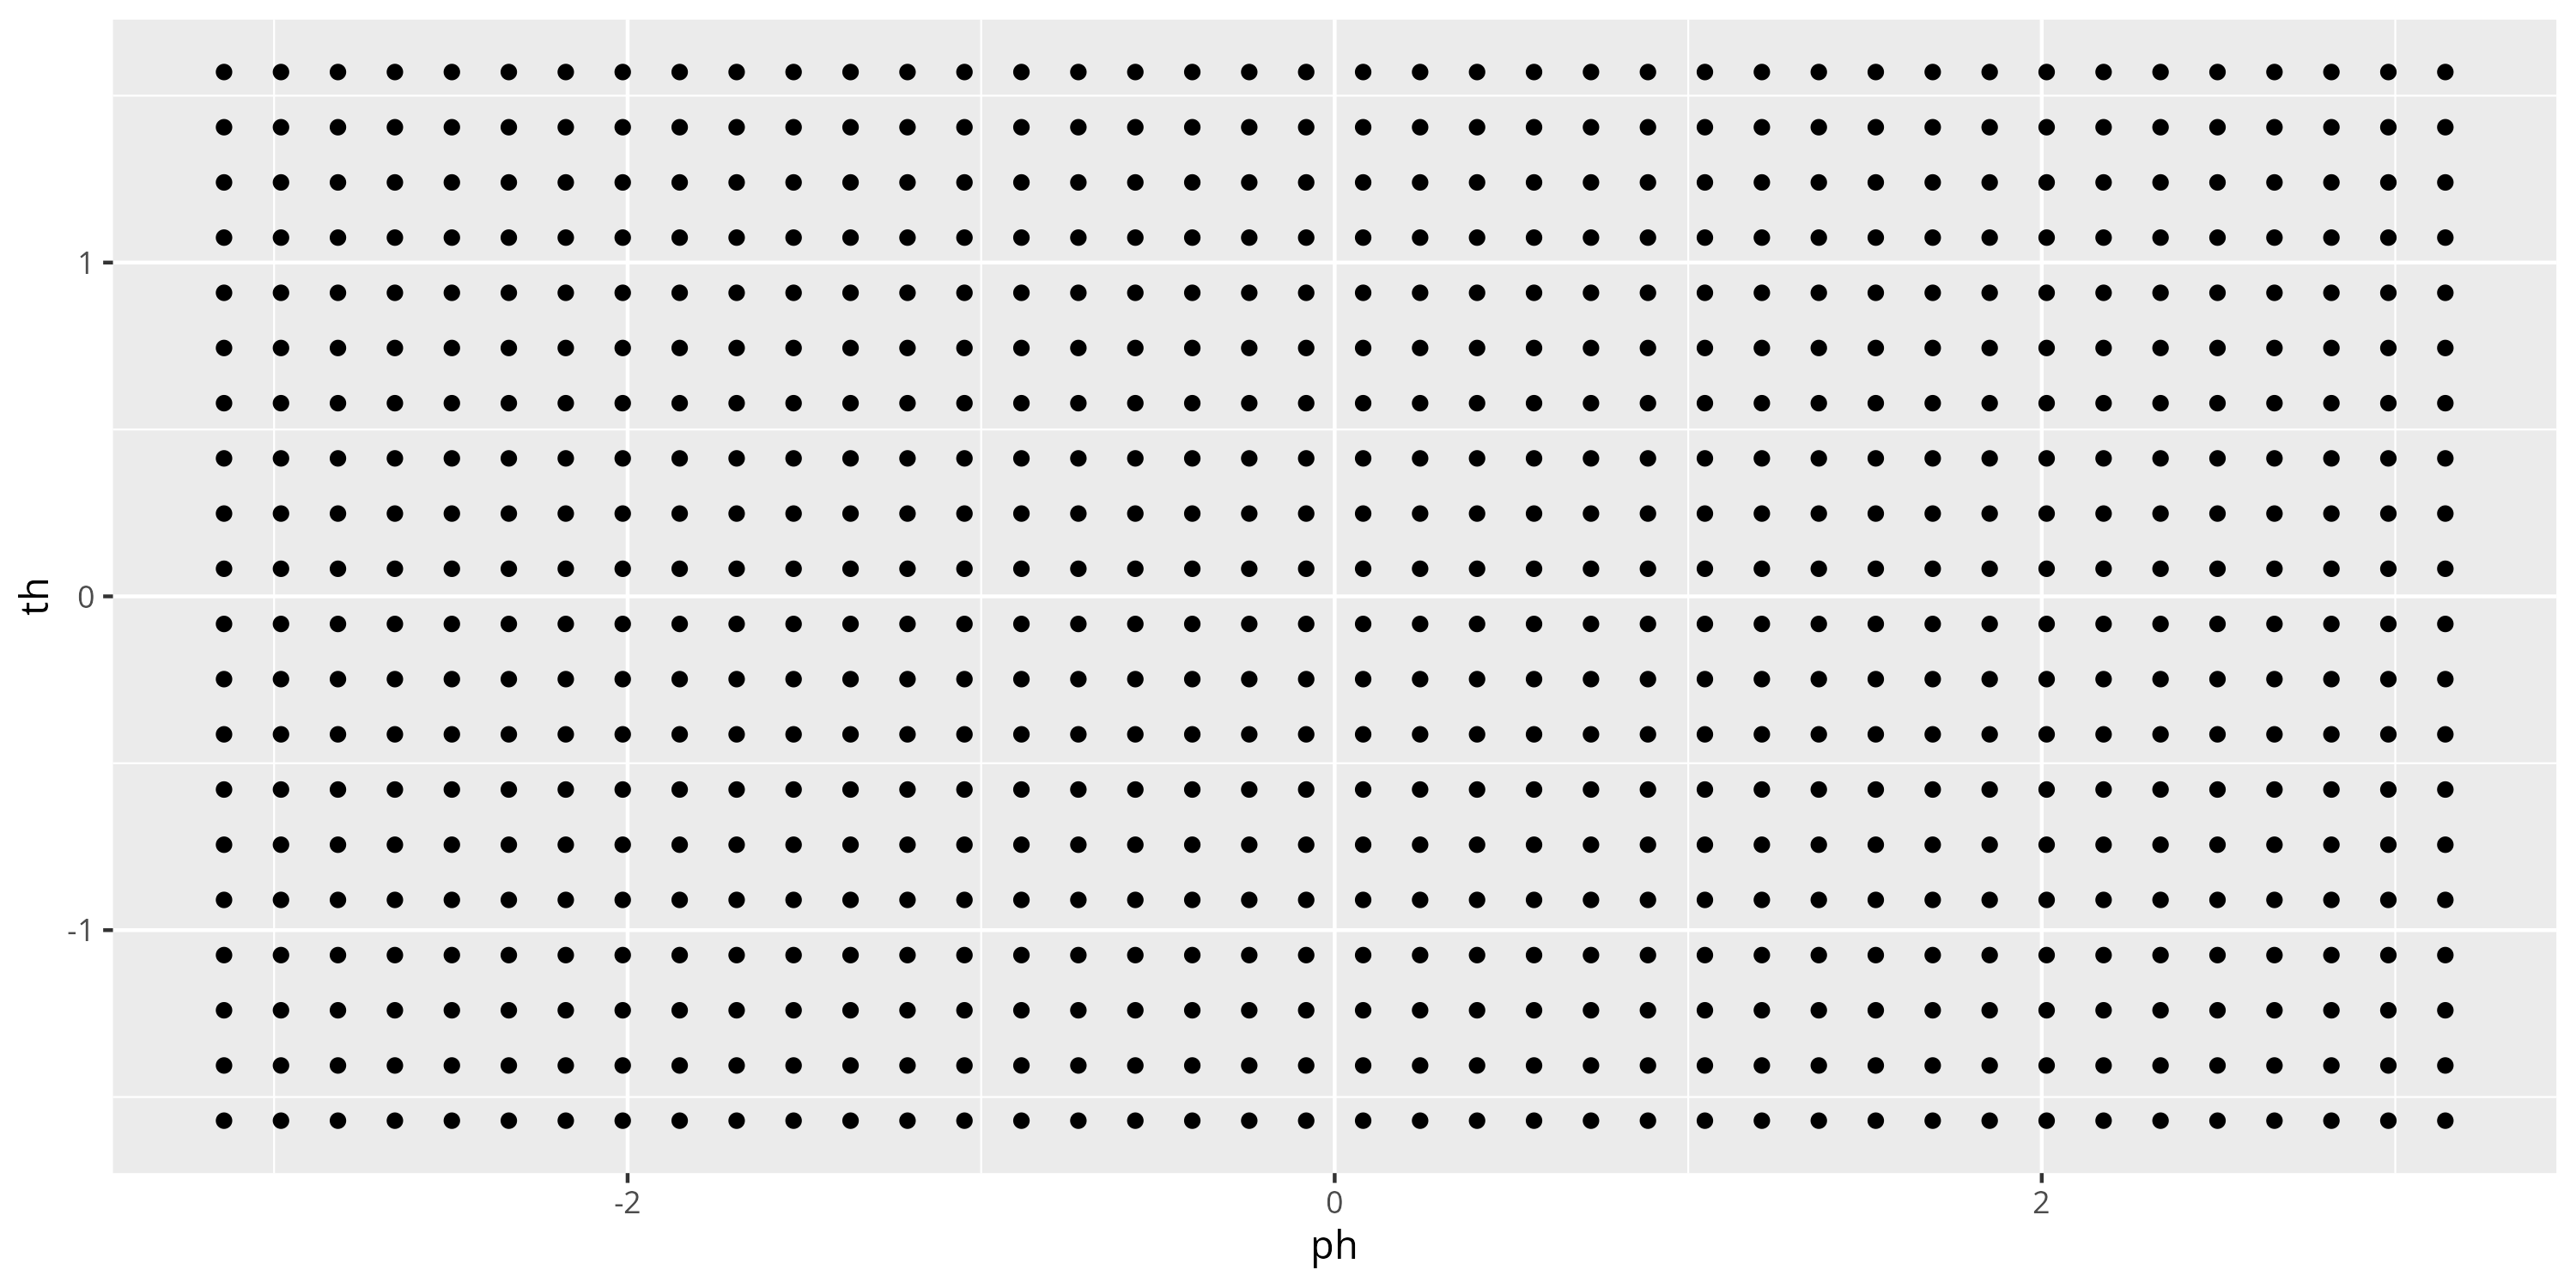
\includegraphics[width=.95\textwidth]{media/discretized_grid.png}
    %   \captionof{figure}{A figure}
      \label{fig:test1}
    \end{minipage}%
    \begin{minipage}{.5\textwidth}
      \centering
      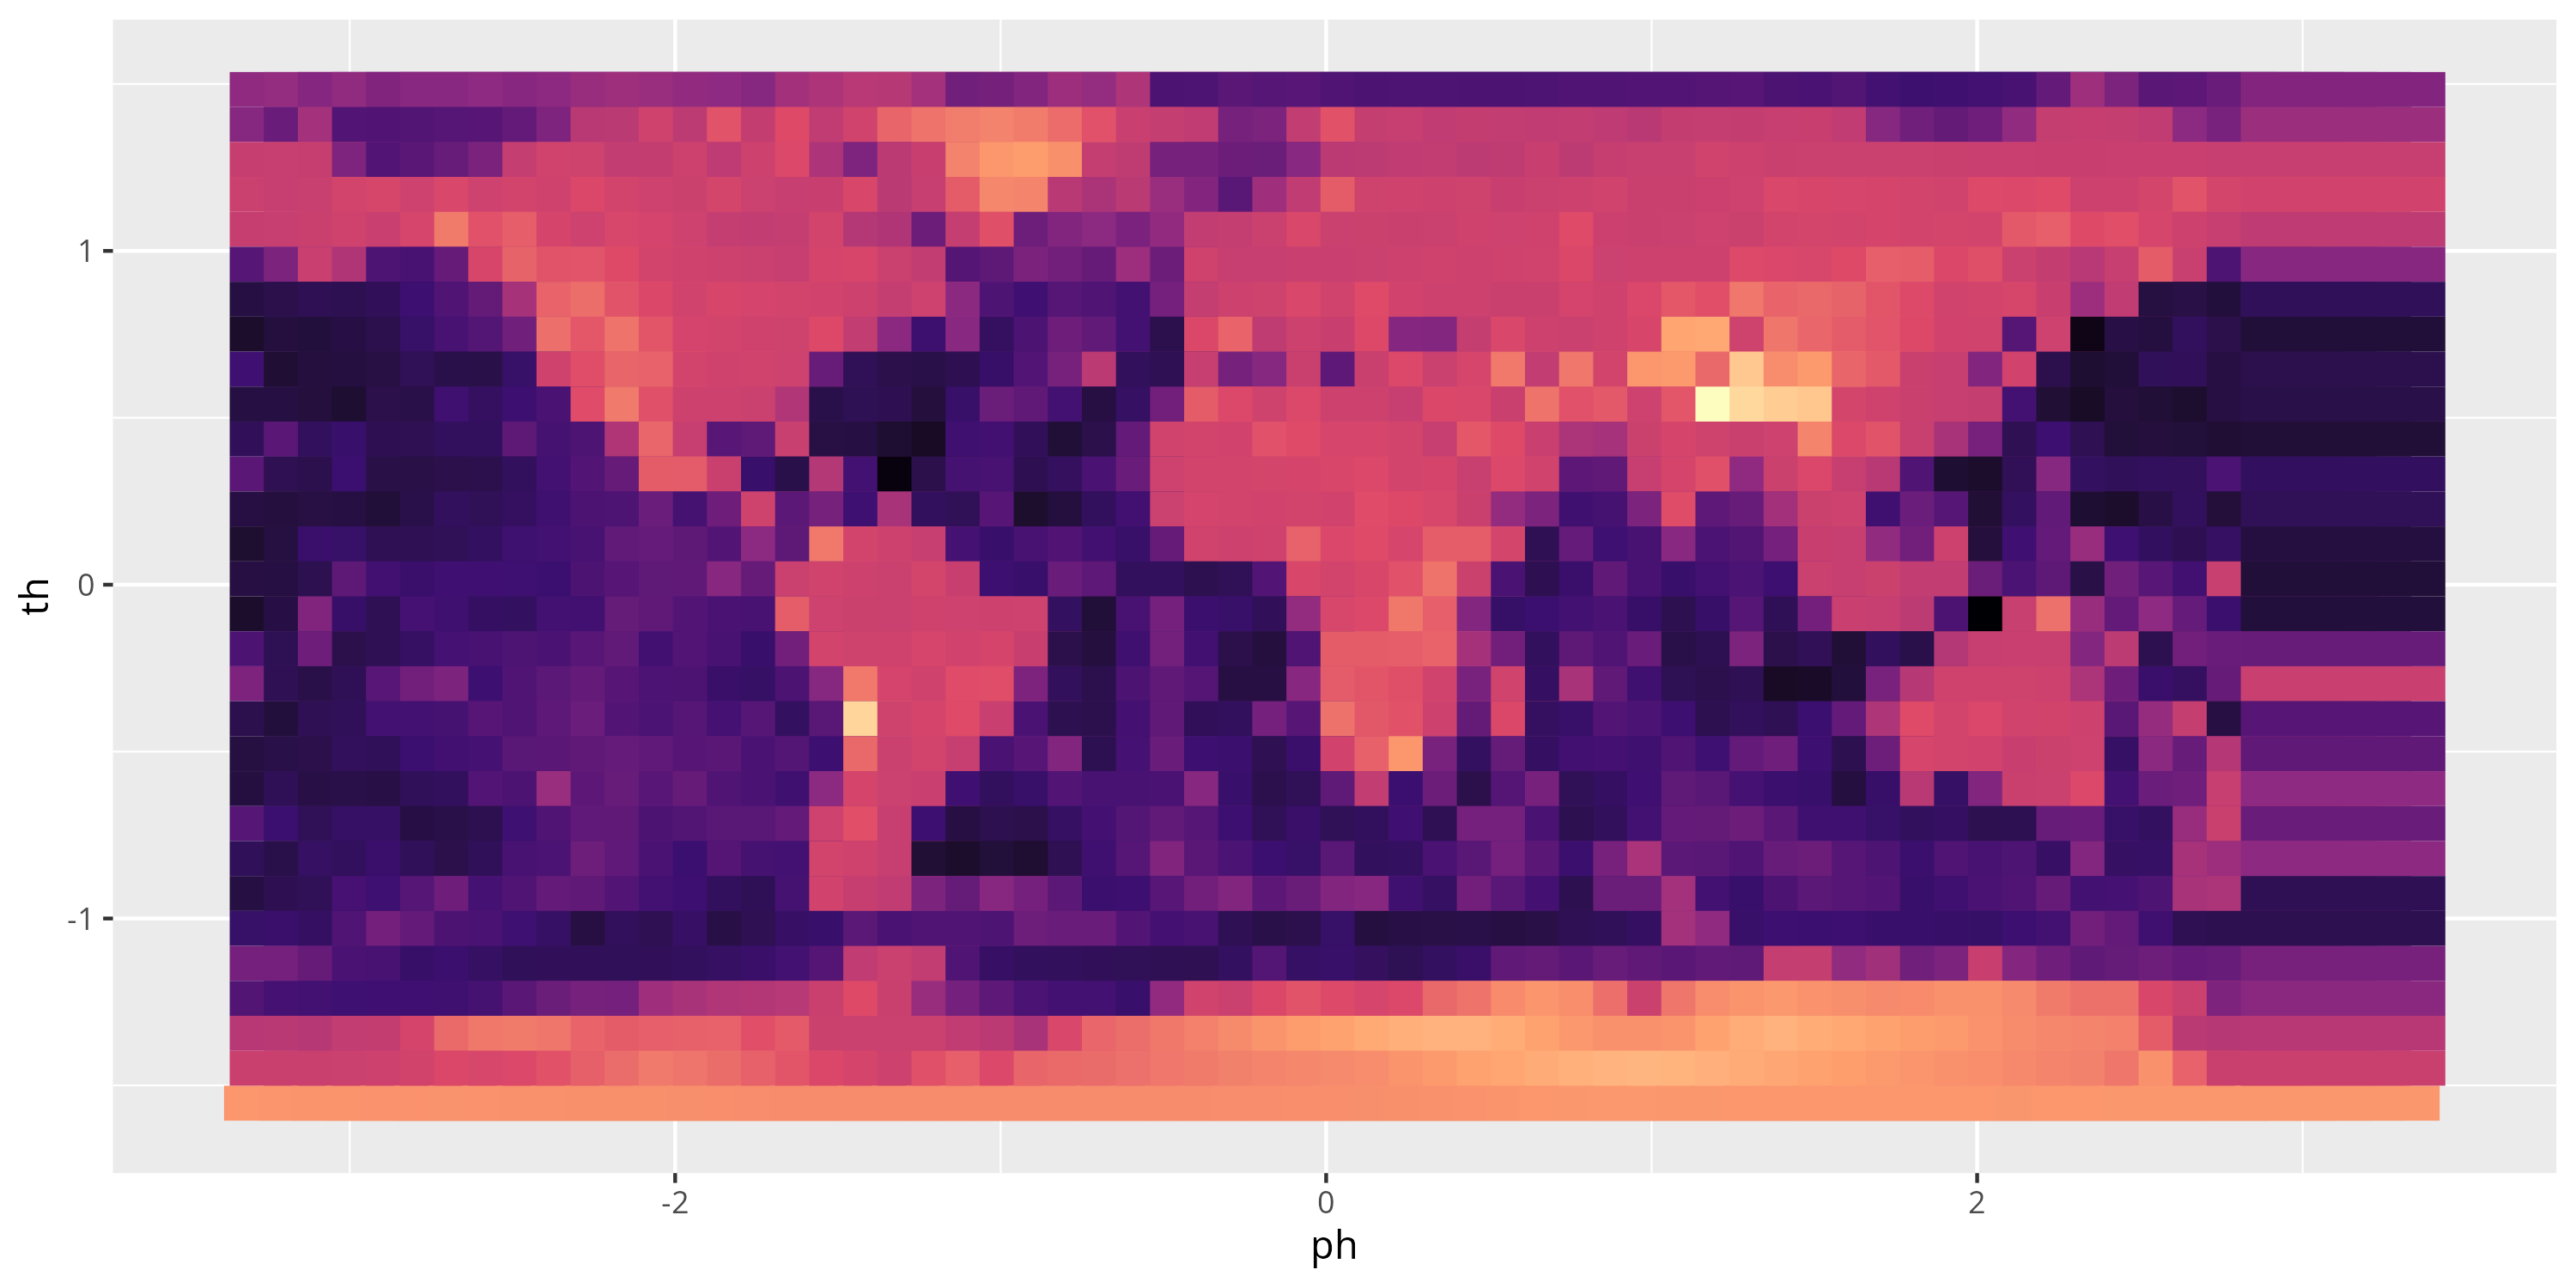
\includegraphics[width=.95\textwidth]{media/discretized_reduced.png}
    %   \captionof{figure}{Another figure}
      \label{fig:test2}
    \end{minipage}
    \caption{Discretization points (left) of a reduced data set with $n_\theta = 20$, $n_\phi = 40$. On the vertical axis we have $\theta \in [-\pi/2, \pi/2]$, or the latitude; On 
    the horizontal axis we have $\phi \in [-\pi, \pi]$, the longitude.}
\end{figure}

Due to the linear spacing, we only need to know the number of points $n_\theta$ and $n_\phi$ to recreate the spherical coordinate pairs provided 
by the data sets, allowing us to decrease the running memory footprint of our program. In order study informative analytics about our model, we first enumerate
the characteristics of each data set.

% \begin{figure}[h!]
    % \centering a
    \begin{center}
    \begin{tabular}{ c |  c  c  c }
        & $n_\theta$ & $n_\phi$ & $N$ \\ 
    \hline
    small & 180 & 360 & 64800\\
    med & 540 & 1080 & 583200\\
    hi \\
    ultra
    \end{tabular}
    \end{center}
% \end{figure}
$$\theta \in [0, \pi],\ \ \phi \in [0, \pi2]$$

We'll use these values later when we study the time it takes to compute our model.

\subsection{Visualization}

\textbf{TODO:} [ ] add 3-d maps

\section{Mathematical Model}

We define $\mathcal{S}_L$ a spherical model of degree $L$ to be the set of coefficients $\{C_0^0, C_1^0, C_1^1, \dots, C_L^L\}$ and \\ 
$\{S_0^0, S_1^0, SL^L, \dots, S_L^L\}$ that are used in conjonction with (\ref{eq:f_iso}) to provide an estimate of $f$, $\hat f$, defined as:
\begin{equation}
    \hat f(\theta, \phi; L) = \sum_{l = 0}^{L}\sum_{m = 0}^l \bar P_l^m(\cos\theta)[C_l^m\cos m\phi + S_l^m \sin m \phi].
\end{equation}

Notice that the $+\infty$ in the outer summation has been replaced with the degree of the model, $L$. We will evaluate the efficacy of the model by studying the distance between $f$ and $\hat f$
at the observations of our data set. Of notable interest will be the average absolute error (AAE) and the mean squared error (MSE):
\begin{equation}
    \label{eq:AAE}
    \mathrm{AAE}(l_{max}) = \frac{1}{N}\sum_{i = 1}^{N} |\hat f_i - f_i |, \quad MSE(l_{max}) = \frac{1}{N} \sum_{i = 1}^N (\hat f_i - f_i)^2
\end{equation}

where $\hat f_i$ denotes the estimated altitude evaluated at the $i$th data point and $f_i$ is the true observed altitude of the $i$th data point.


\subsection{Computation of Coefficients via Numerical Integration}


    
We approximate the Laplace Series coefficients via a 2 dimensional analogue of the rectangle rule.  
\begin{align*}
    C_l^m &\approx \sum_{i = 1}^{n_\phi}\sum_{j = 1}^{n_\theta} f(\theta_j, \phi_i) P_l^m (\cos \theta_j)\cos (m \phi_i) \sin \theta_j \Delta\theta \Delta\phi\\
          &\approx \Delta\theta \Delta\phi\sum_{i = 1}^{n_\phi}\cos (m \phi_i)\sum_{j = 1}^{n_\theta} f(\theta_j, \phi_i) P_l^m (\cos \theta_j) \sin \theta_j\\
    S_l^m &\approx \sum_{i = 1}^{n_\phi}\sum_{j = 1}^{n_\theta} f(\theta_j, \phi_i) P_l^m (\cos \theta_j)\sin (m \phi_i) \sin \theta_j \Delta\theta \Delta\phi\\
          &\approx \Delta\theta \Delta\phi\sum_{i = 1}^{n_\phi}\sin (m \phi_i)\sum_{j = 1}^{n_\theta} f(\theta_j, \phi_i) P_l^m (\cos \theta_j) \sin \theta_j
\end{align*}

This method computes \textit{individual} Laplace series coefficients in $O(N)$ time! Thus, computing the coefficients for a Discrete Laplace Series (DLS) of order $l$ runs in
$O(Nl^2)$. More interestingly, each $C_l^m$ or $S_l^m$ can be computed \textbf{independently} of any other coefficient. Whereas solving the linear least squares problem requires computing
every $C_l^m$ and $C_l^m$ up to a given $L$ in a single operation, this method allows us the ability to compute any arbitrary $C_l^m$ directly. Why do we care? If I alraedy have the first 500 $C_l^m$ coefficients computed
and stored in a text file, I can \textit{directly} compute the next p coefficients in $O(pN)$ time. This method allows us to also compute ranges of $C_l^m$ and $S_l^m$ without messing around
with bulky matrices taking up millions of bytes. As a consequence, there are simple yet powerful parallelization schemes that can be easily implemented to speed up computation and increase 
the performance of our models.

% \newpage
\subsection{Comparison with Linear Squares}

Let's start by exploring the small data set and benchmarking how long it takes to compute a model of degree $l$ for $l \in \{0, 2, 4, \dots, 20\}$ via 
a) an overdetermined system of linear equations b) numerical integration. Our aim in this section is to show that computing the coefficients via numerical integration
provides numerous benefits to the overall methodology and allows us to compute higher degree models with lower error more efficiently.

\subsubsection{Timing}


We experimentally corroborate the theoretical hypothesis that the least squares computation is of time complexity $O(Nl^4)$ for a data set of size $N$ and 
model degree $l$.

\begin{figure}[h!]
    \centering
    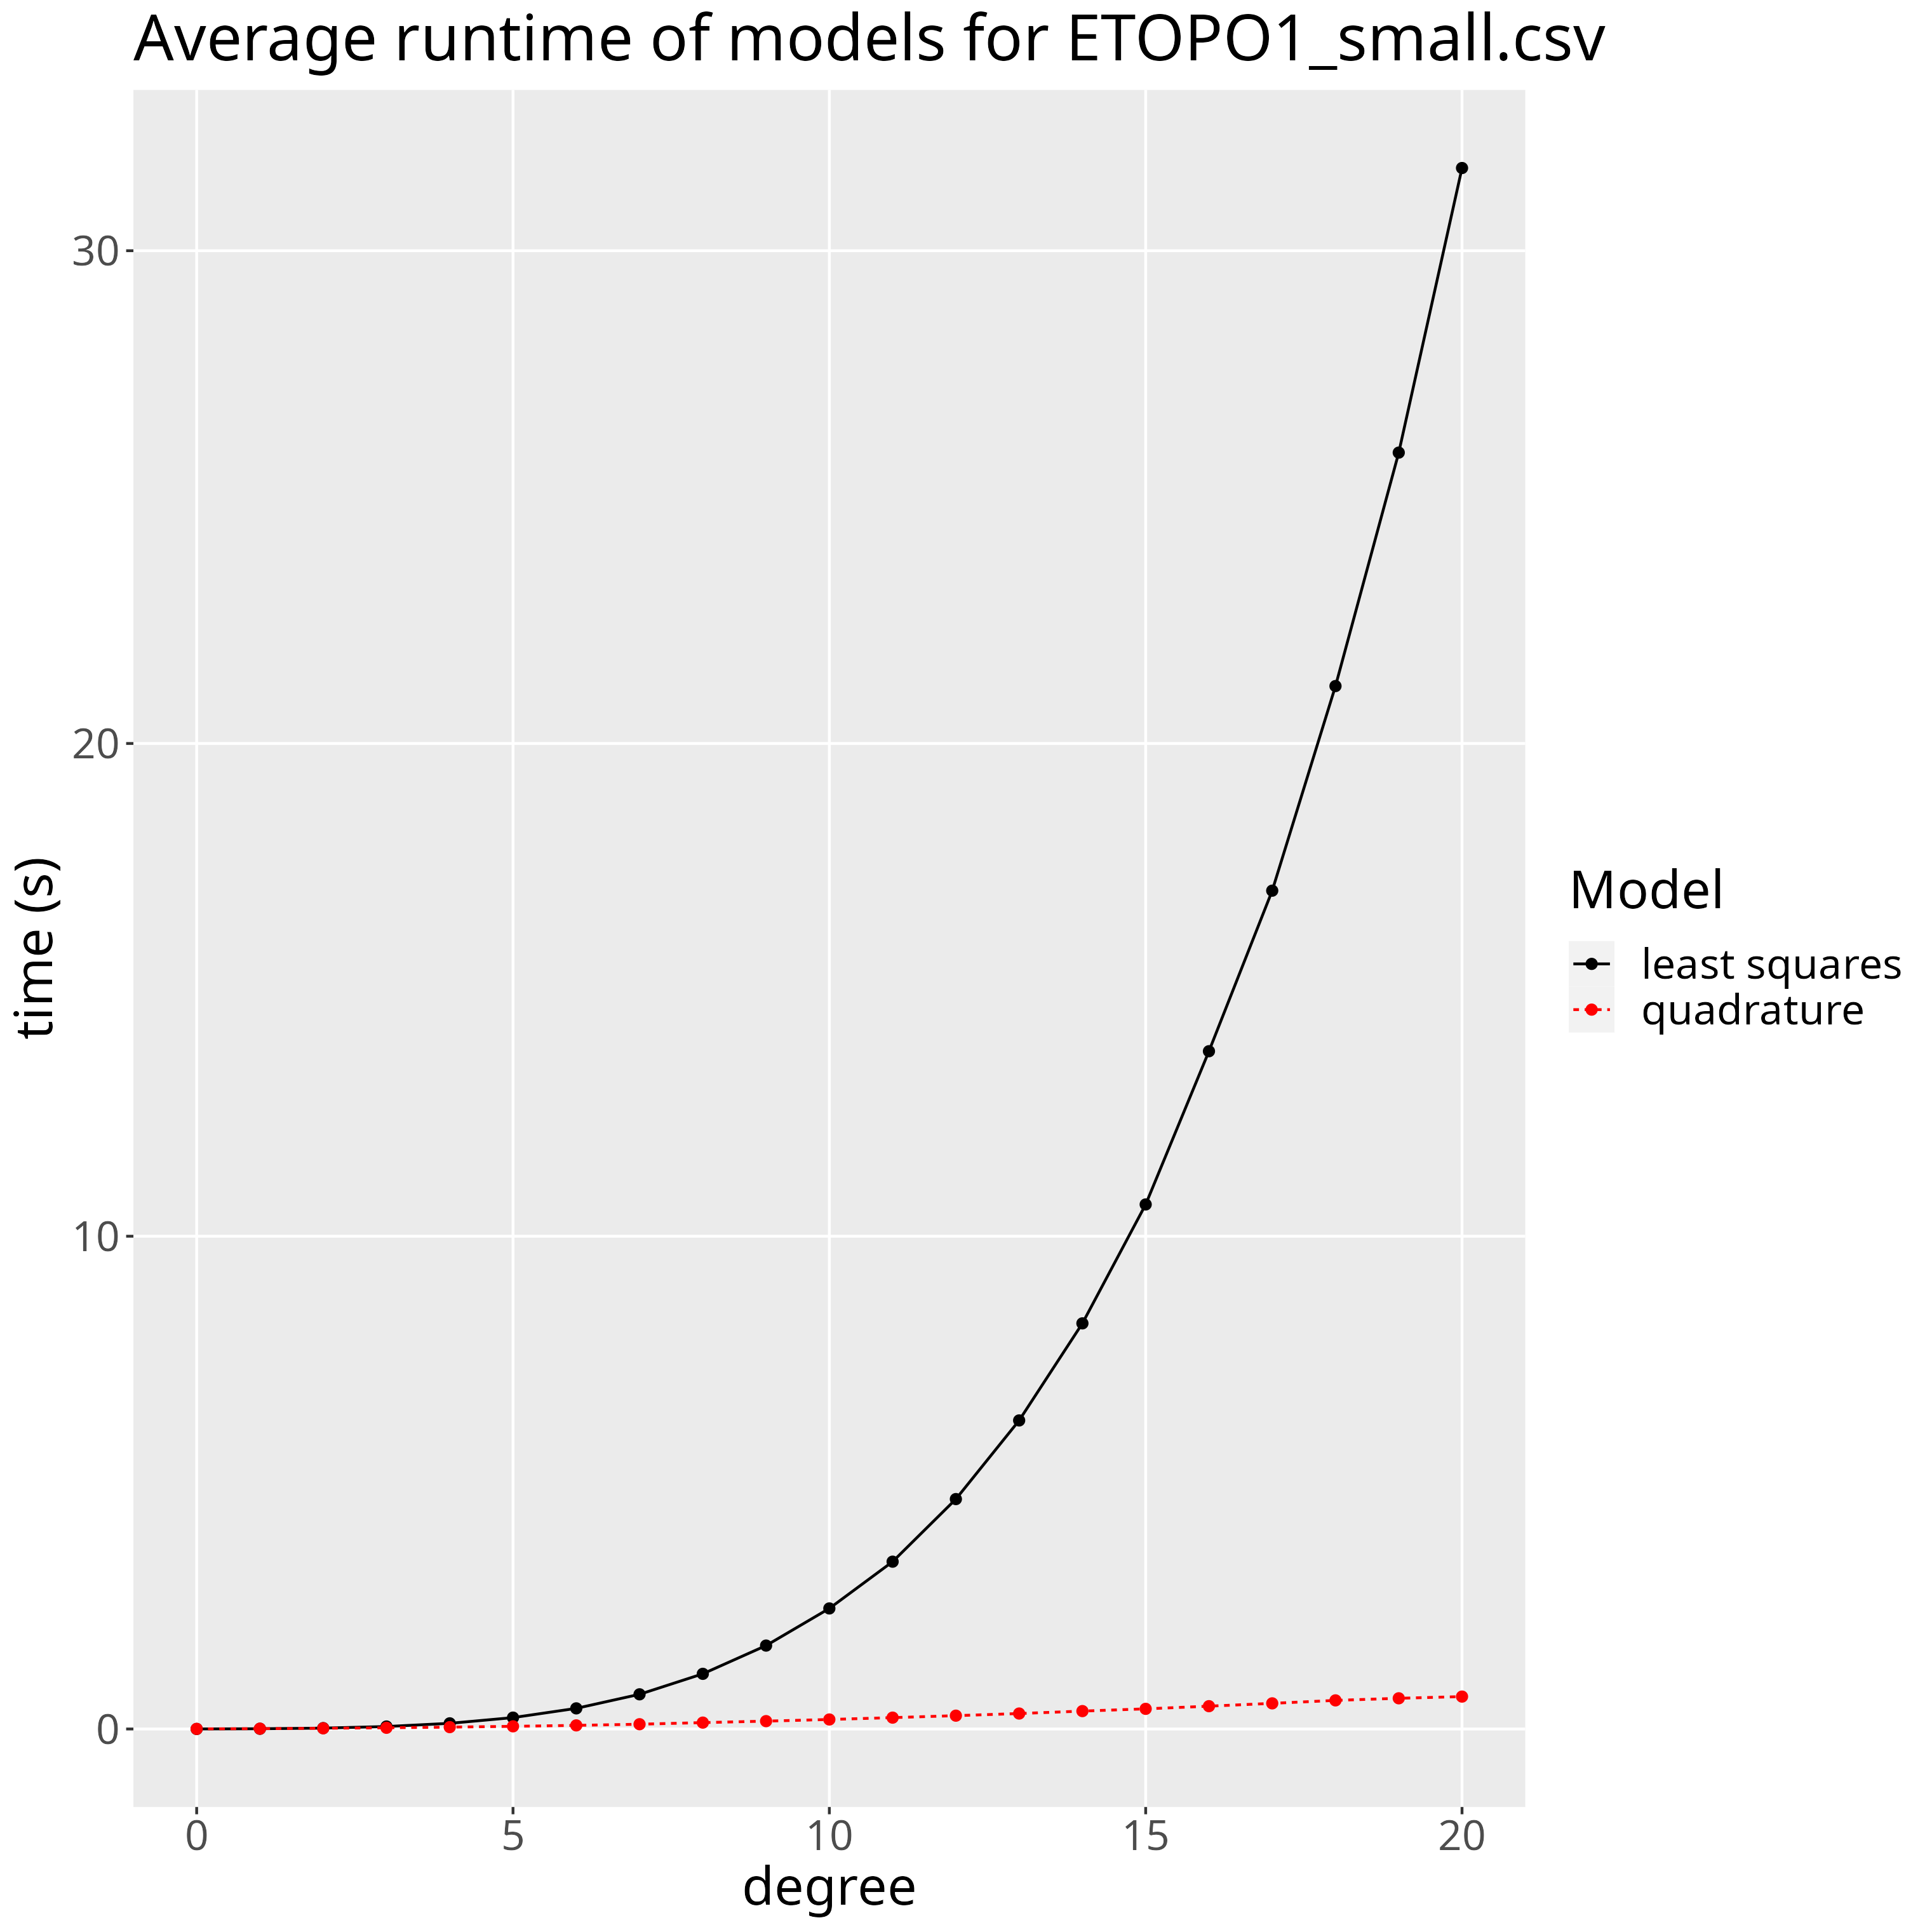
\includegraphics[width=0.5\textwidth]{media/average_runtime.png}
    \caption{A timing comparison between least squares $\in O(Nl^4)$ and numerical quadrature $\in O(Nl^2)$ to compute the coefficients $C_l^m$ and $S_l^m$ for the small ETOPO1 data set. 
    For each degree of the model Laplace coefficients were computed 5 times. Programs were run in sequential with 1 processor. TODO: Run a linear regression}
    \label{fig:runtime}
\end{figure}


When we study how long it takes to compute a model of degree 20 (Figure \ref{fig:runtime}) for the small data set we find that the least squares method takes, on average, a staggering 31.678 seconds to run. 
Coefficients computed by numerical integration, on the other hand, were generated with an average runtime of 0.656s across
5 trials. As we will see in the following analysis, a model of degree 20 is wholly incomplete to accurately represent a data set with 648000 points, and we are not 
satisfied with the runtime of the least squares method. And that's just for a small $l$. Running the algorithm in sequential for higher values of $l$ would quickly become
intractable due to its steep algorithmic complexity, especially magnified if we wanted to compute models for larger data set with millions of points (The medium data set has half a million) For a model of degree 20, numerical quadrature ran on average ~50x faster than its least squares counterpart. As the degree
of the model increases, so does the disparity between the two runtimes; at $l=20$ our algorithm runs 50 times faster but at $l = 100$ our algorithm could be running 1250 times faster.

Clearly the proposed numerical integration model is faster. But how do two models compare when it comes to average squared error? 


\newpage
\subsubsection{Model Performance}

In the least squares model, coefficients are carefully selected by minimizing the MSE of the prediction, which amounts to solving a linear system in $O(Nl^4)$ time. We are therefore,
by construction, finding optimal coefficients that should miniimze the MSE. We compare how the average abs error, the AAE, varies with
respect to the degree of the model.


\begin{figure}[h!]
    \centering
    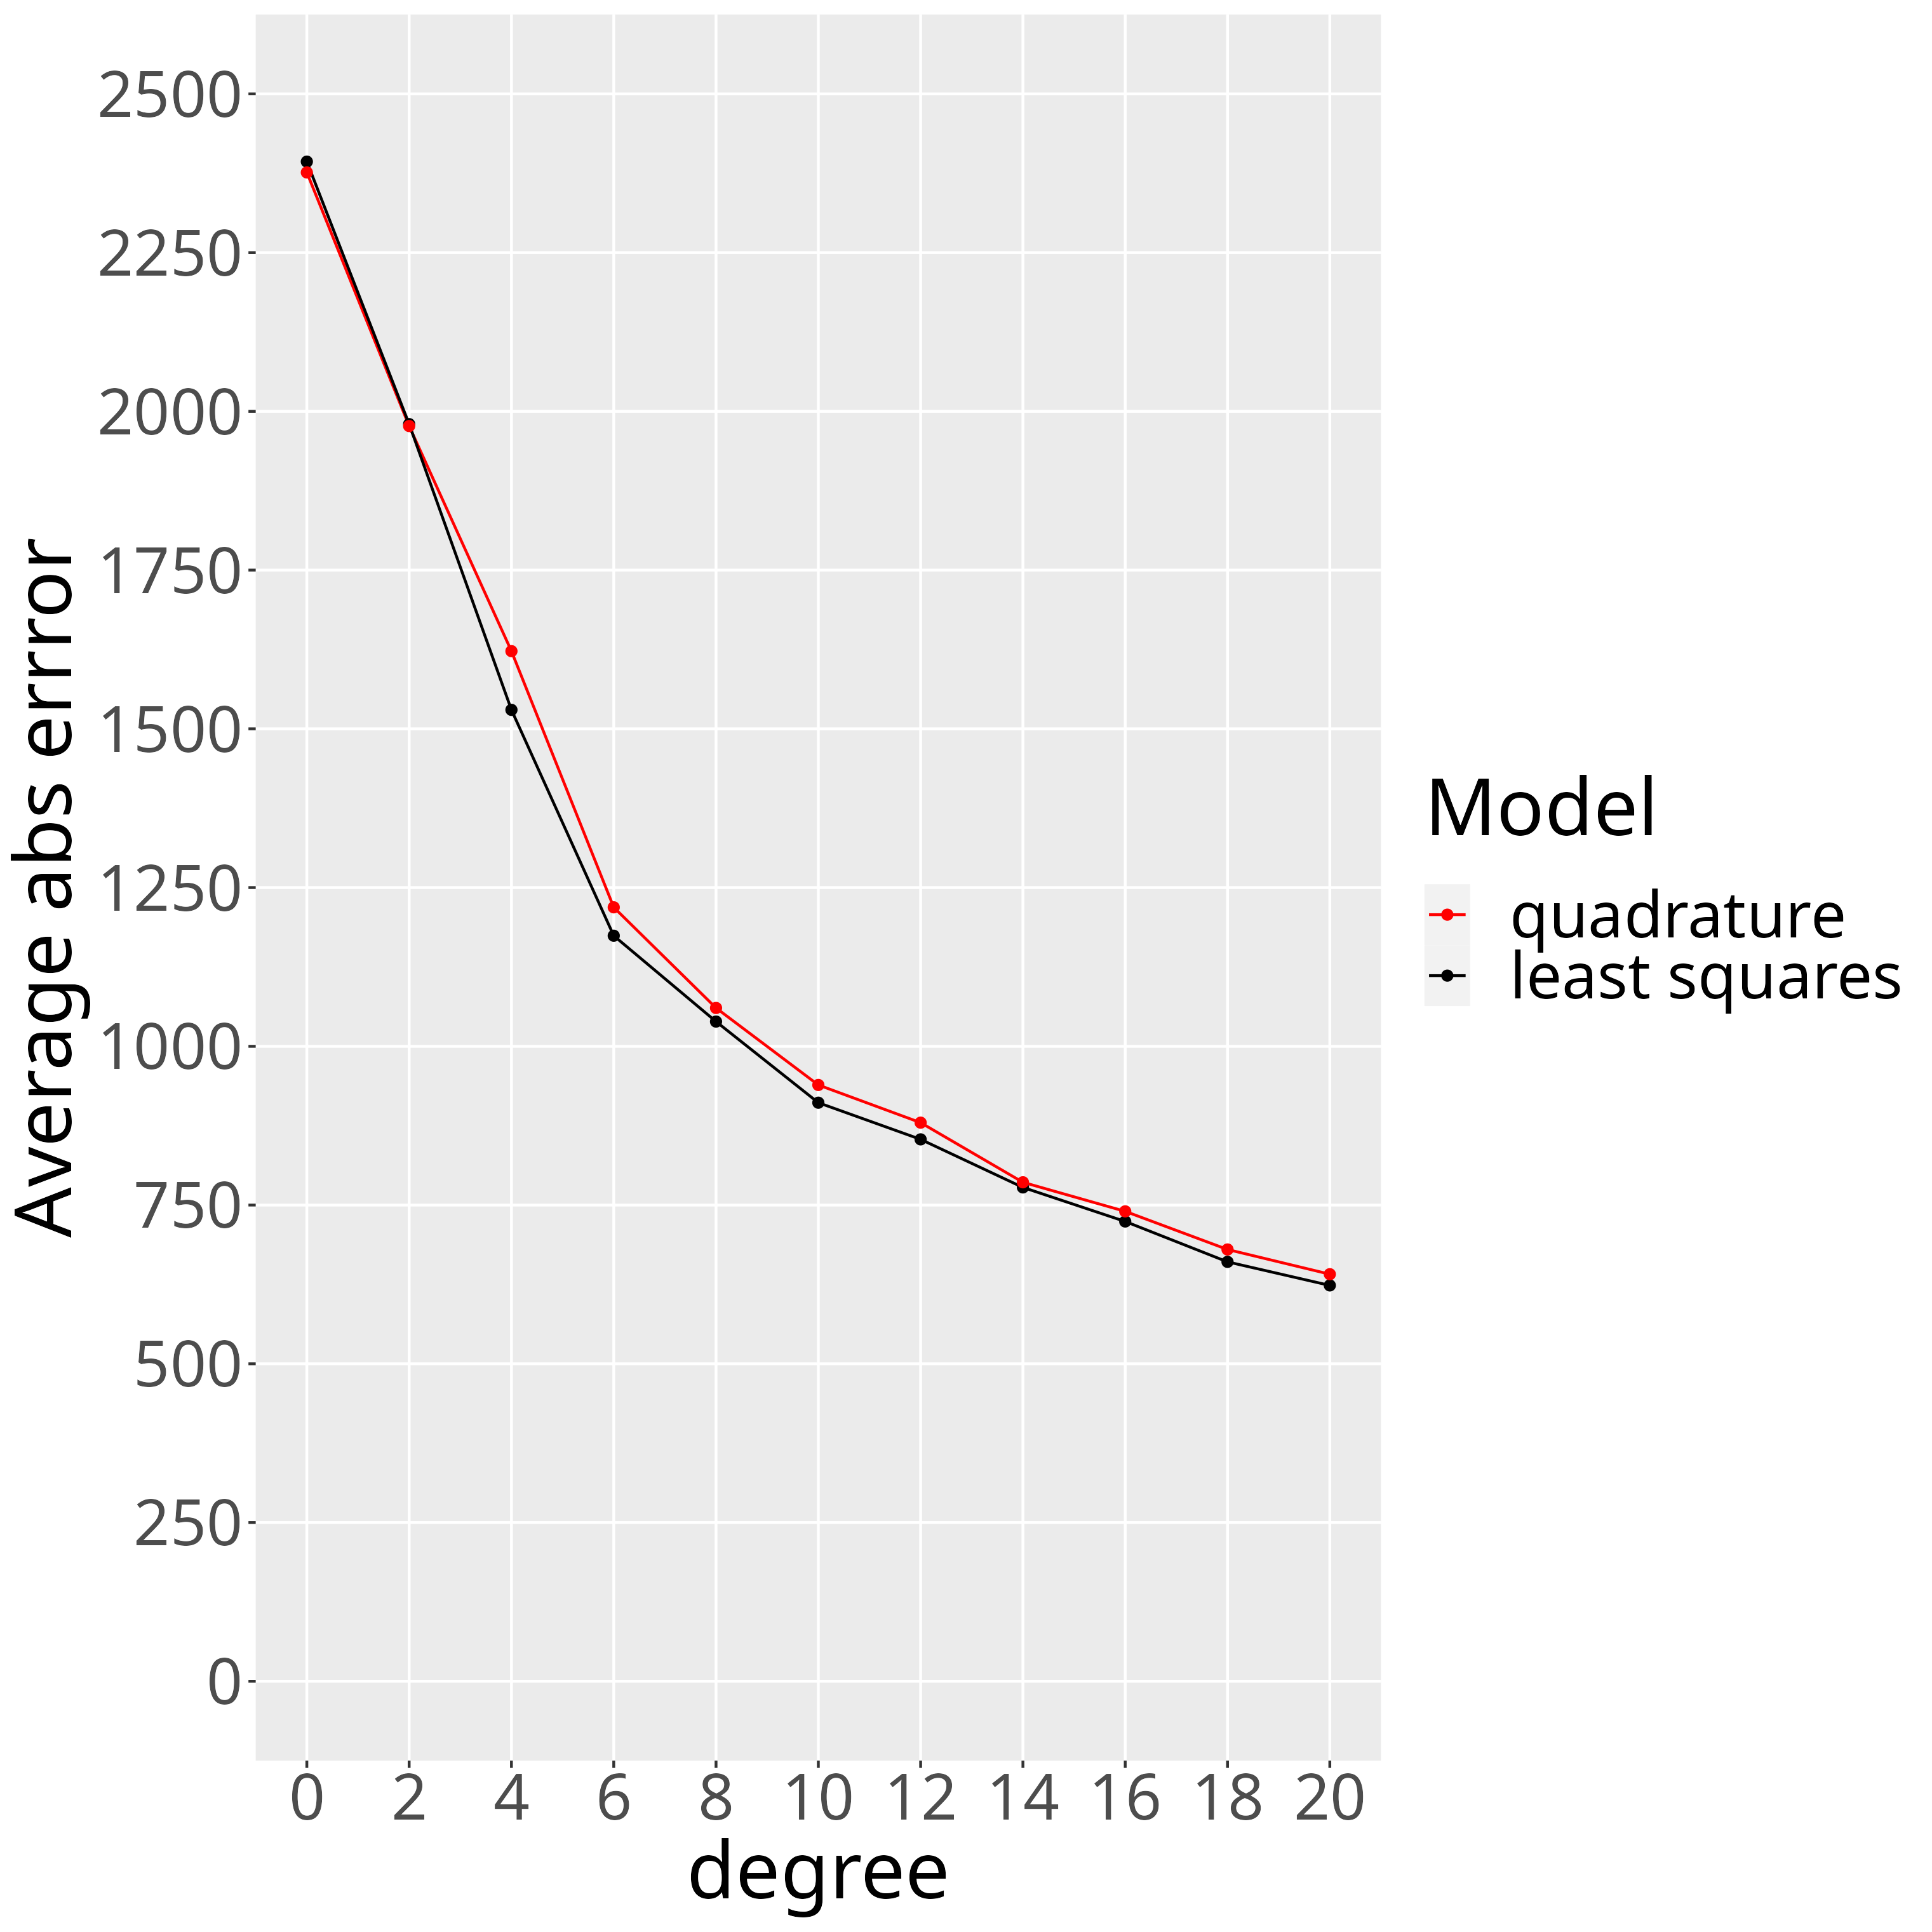
\includegraphics[width=0.6\textwidth]{media/diff_error.png}
    \caption{A Comparison between the average abs error between the least squares estimate and numerical quadrature estimate for the small ETOPO1 data set. Coefficients computed via least squares
    perform slightly better than their quadrature counter parts.}
    \label{fig:erorr}
\end{figure}

Perhaps surprisignly, we find that there is no significant penalty to using numerical quadrature to estimate a model's coefficients. In fact, computing the coefficients via quadrature allows us to 
create higher degree models that, running in the same time as a low-order least squares model, will have far lower average absolute error values and furthermore the distributions of the error will be
much tighter, exhibiting lower variance. In fact, as will be shown in the next section, we can run a degree 200 model using numerical integration in around 20 seconds whose average abs error
is 148.76, compared to the degree 20 model whos AAE is 641.1.

\subsubsection{Higher Degree Models}
In this section we explore the distribution of error values ($\hat f - f$) for models up to degree $l = 300$, computed for the small, medium, and high resolution data sets.

We start off by showing the evolution of the model's estimates as the degree $l$ increases

\begin{figure}[h!]
    \begin{minipage}{.245\textwidth}
        \centering
        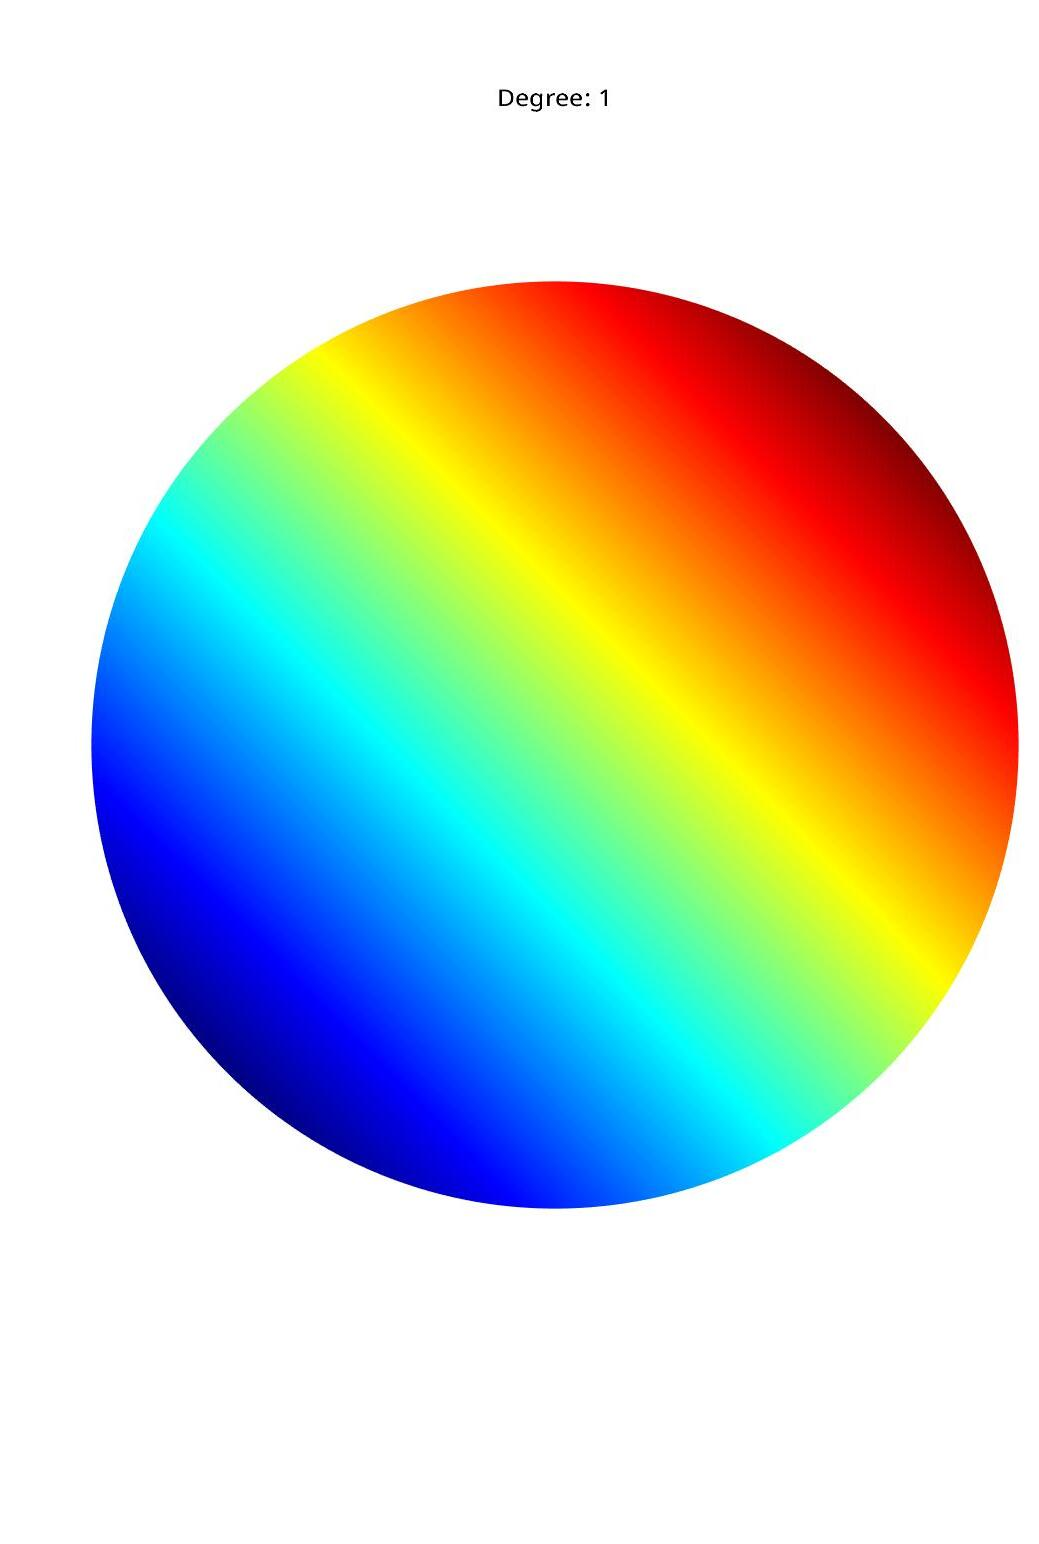
\includegraphics[width=0.95\linewidth]{media/med_1.jpg}
        \label{fig:med1}
    \end{minipage}
    \begin{minipage}{.245\textwidth}
        \centering
        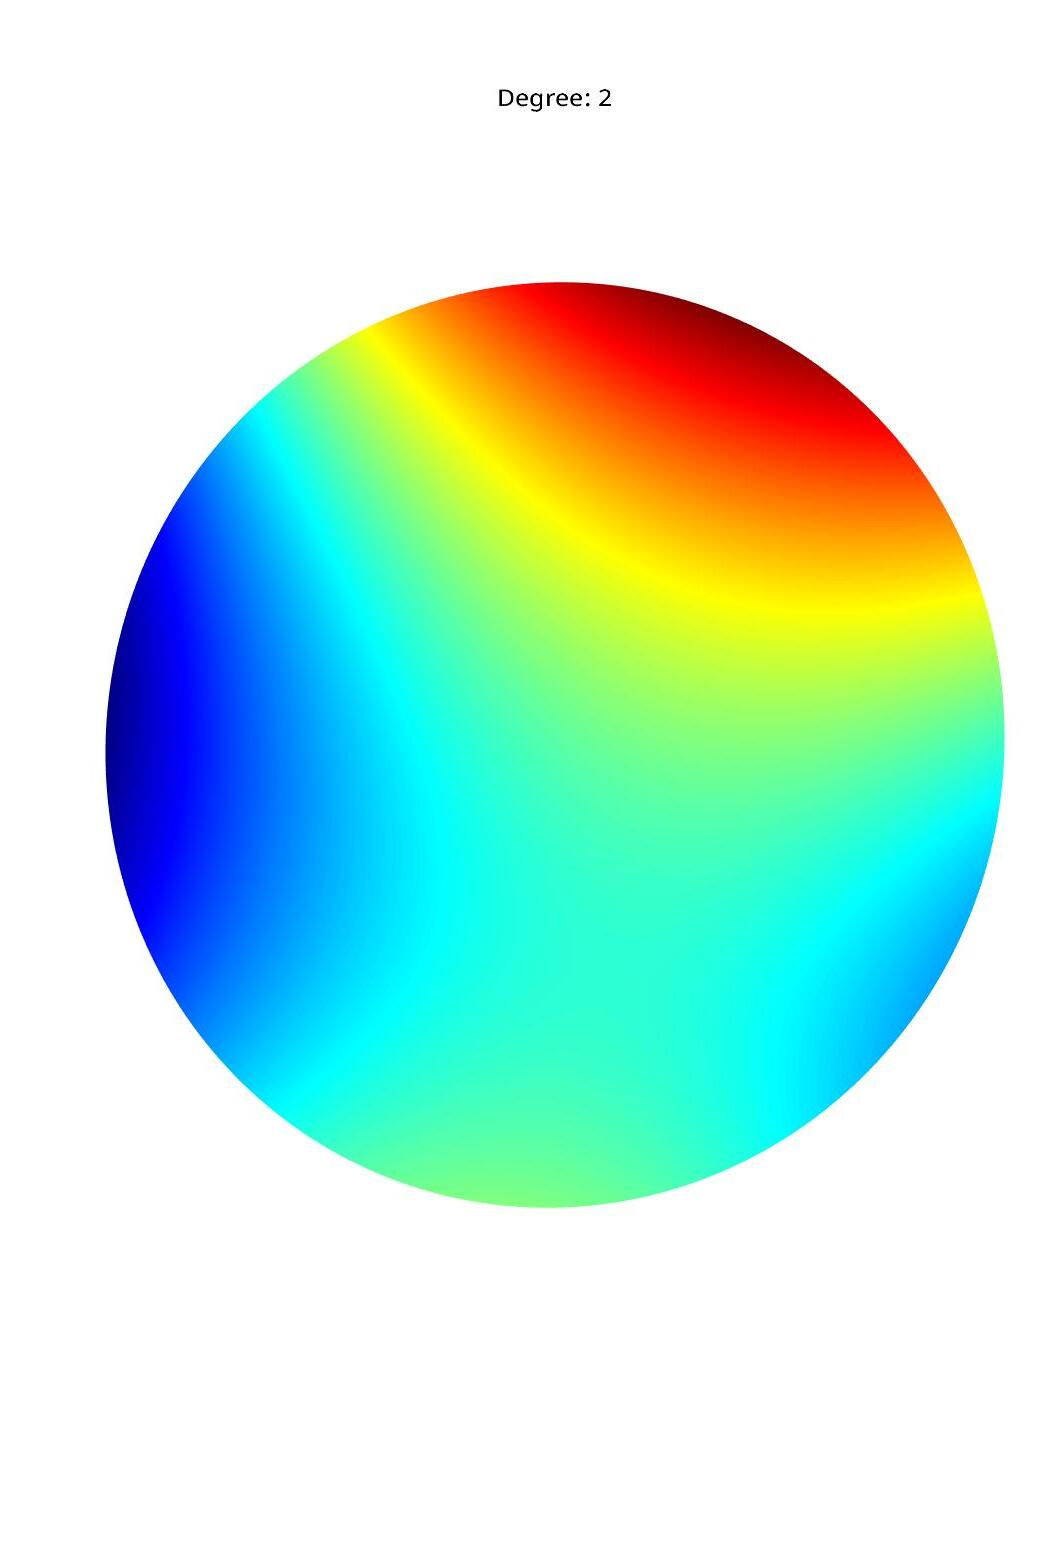
\includegraphics[width=0.95\linewidth]{media/med_2.jpg}
        \label{fig:med2}
    \end{minipage}
    \begin{minipage}{.245\textwidth}
        \centering
        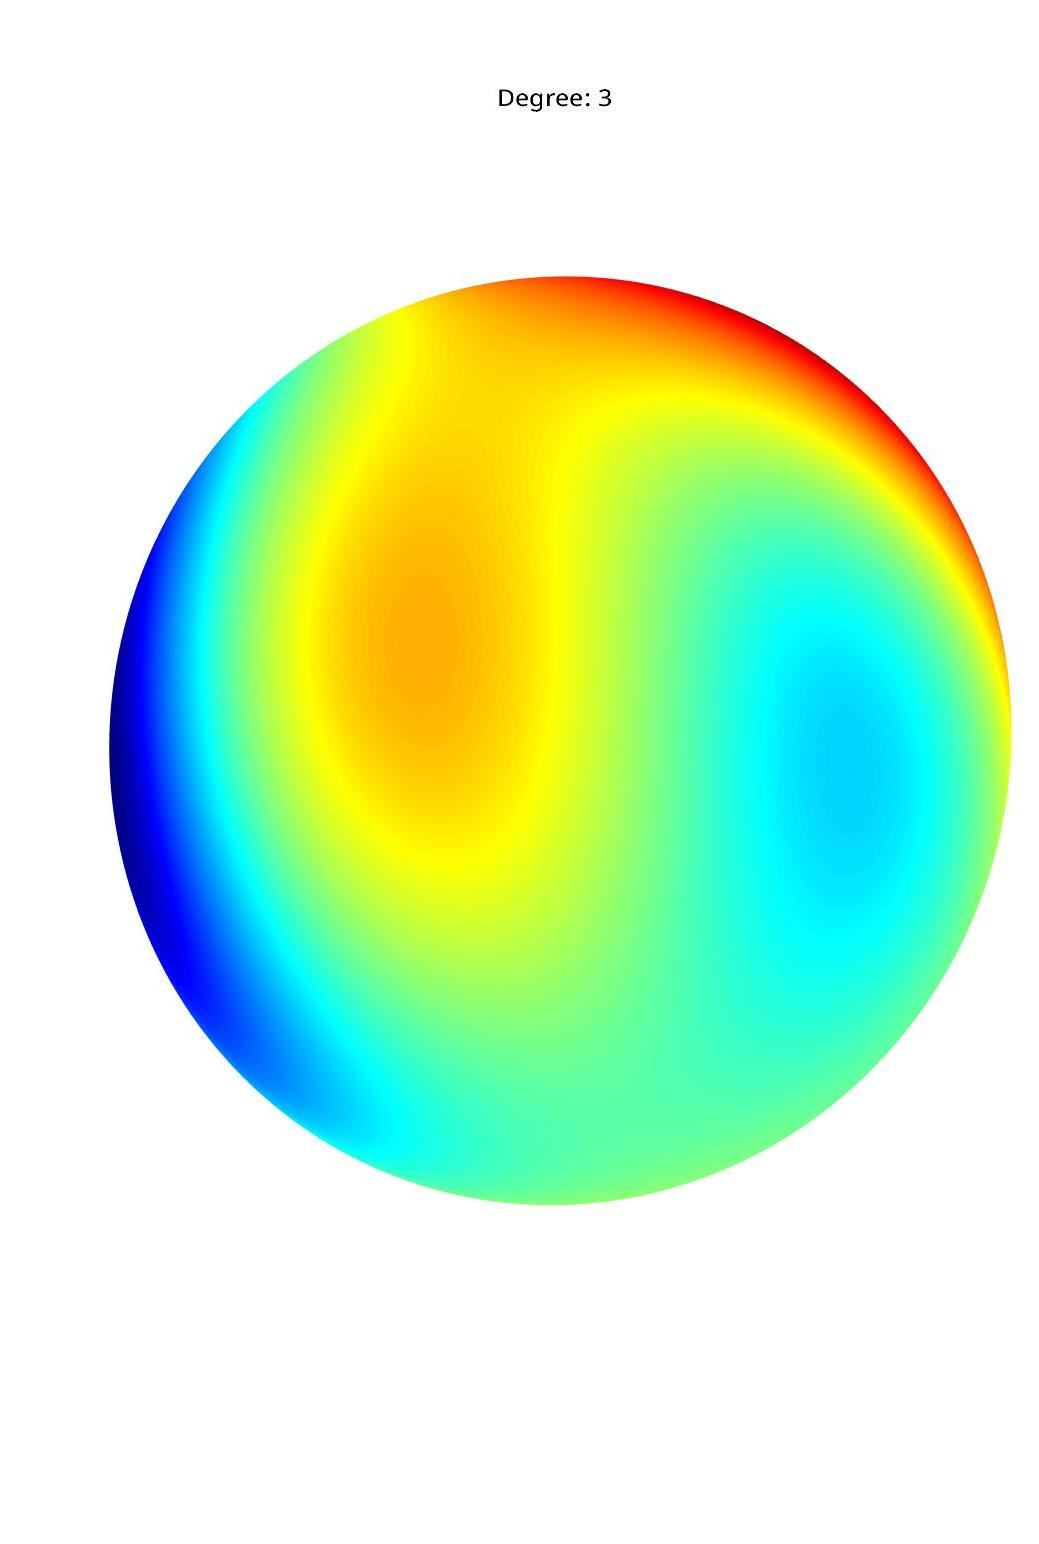
\includegraphics[width=0.95\linewidth]{media/med_3.jpg}
        \label{fig:med3}
    \end{minipage}
    \begin{minipage}{.245\textwidth}
        \centering
        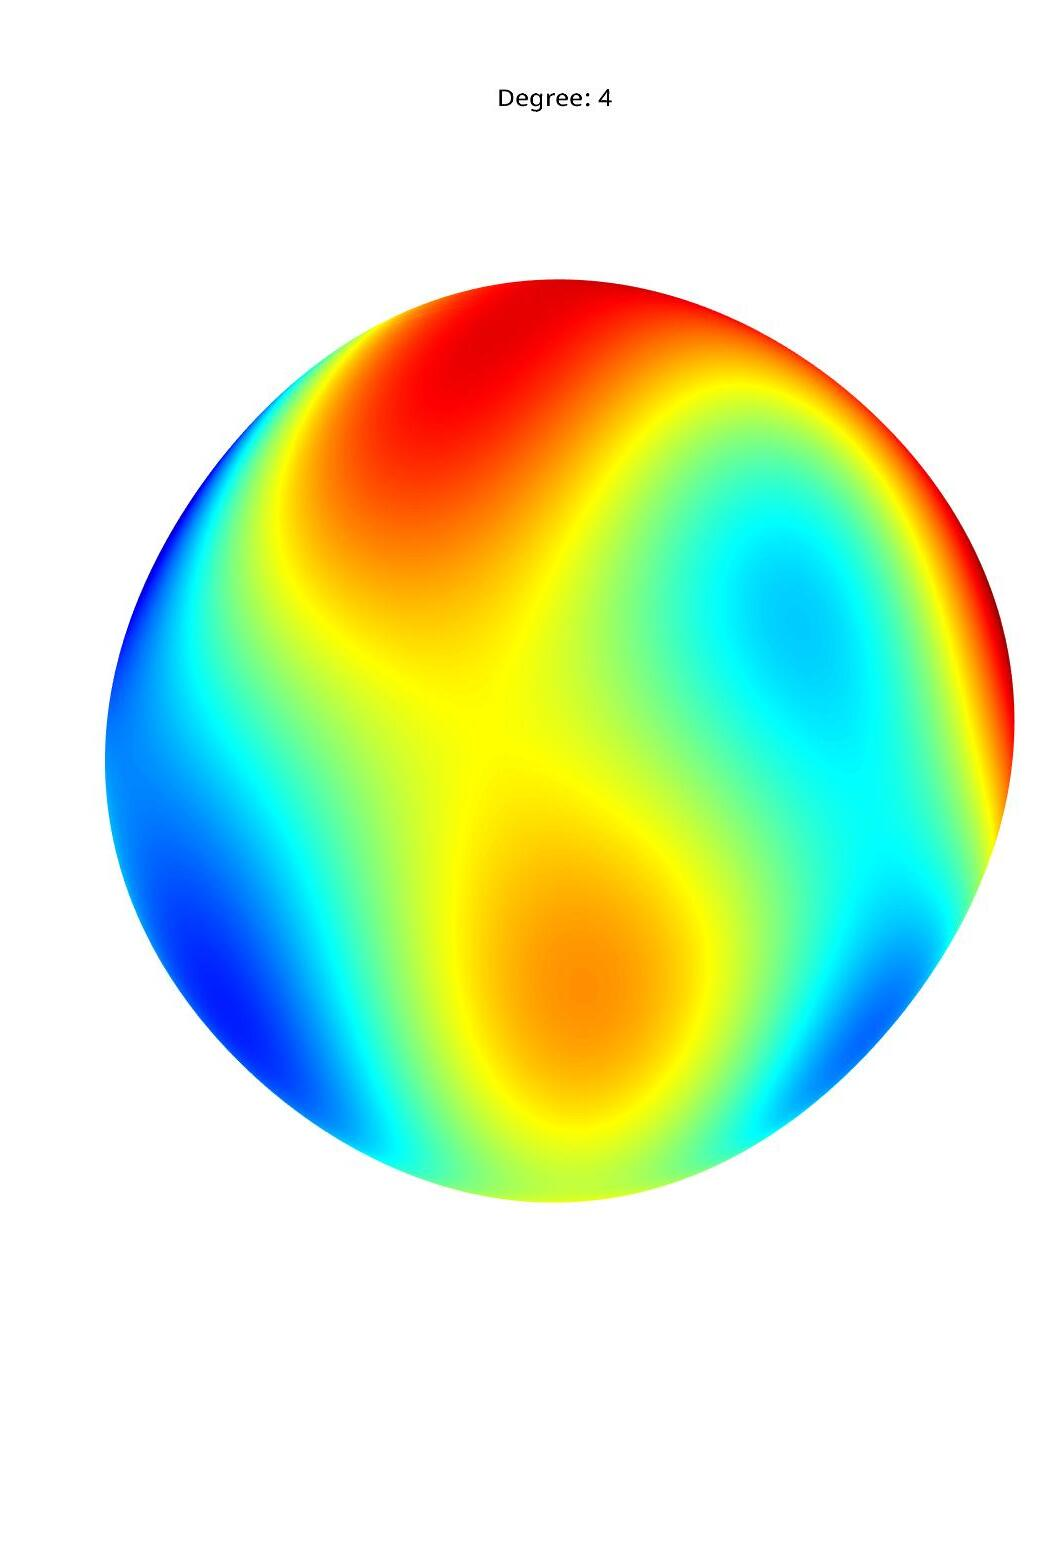
\includegraphics[width=0.95\linewidth]{media/med_4.jpg}
        \label{fig:med4}
    \end{minipage}
    \begin{minipage}{.245\textwidth}
        \centering
        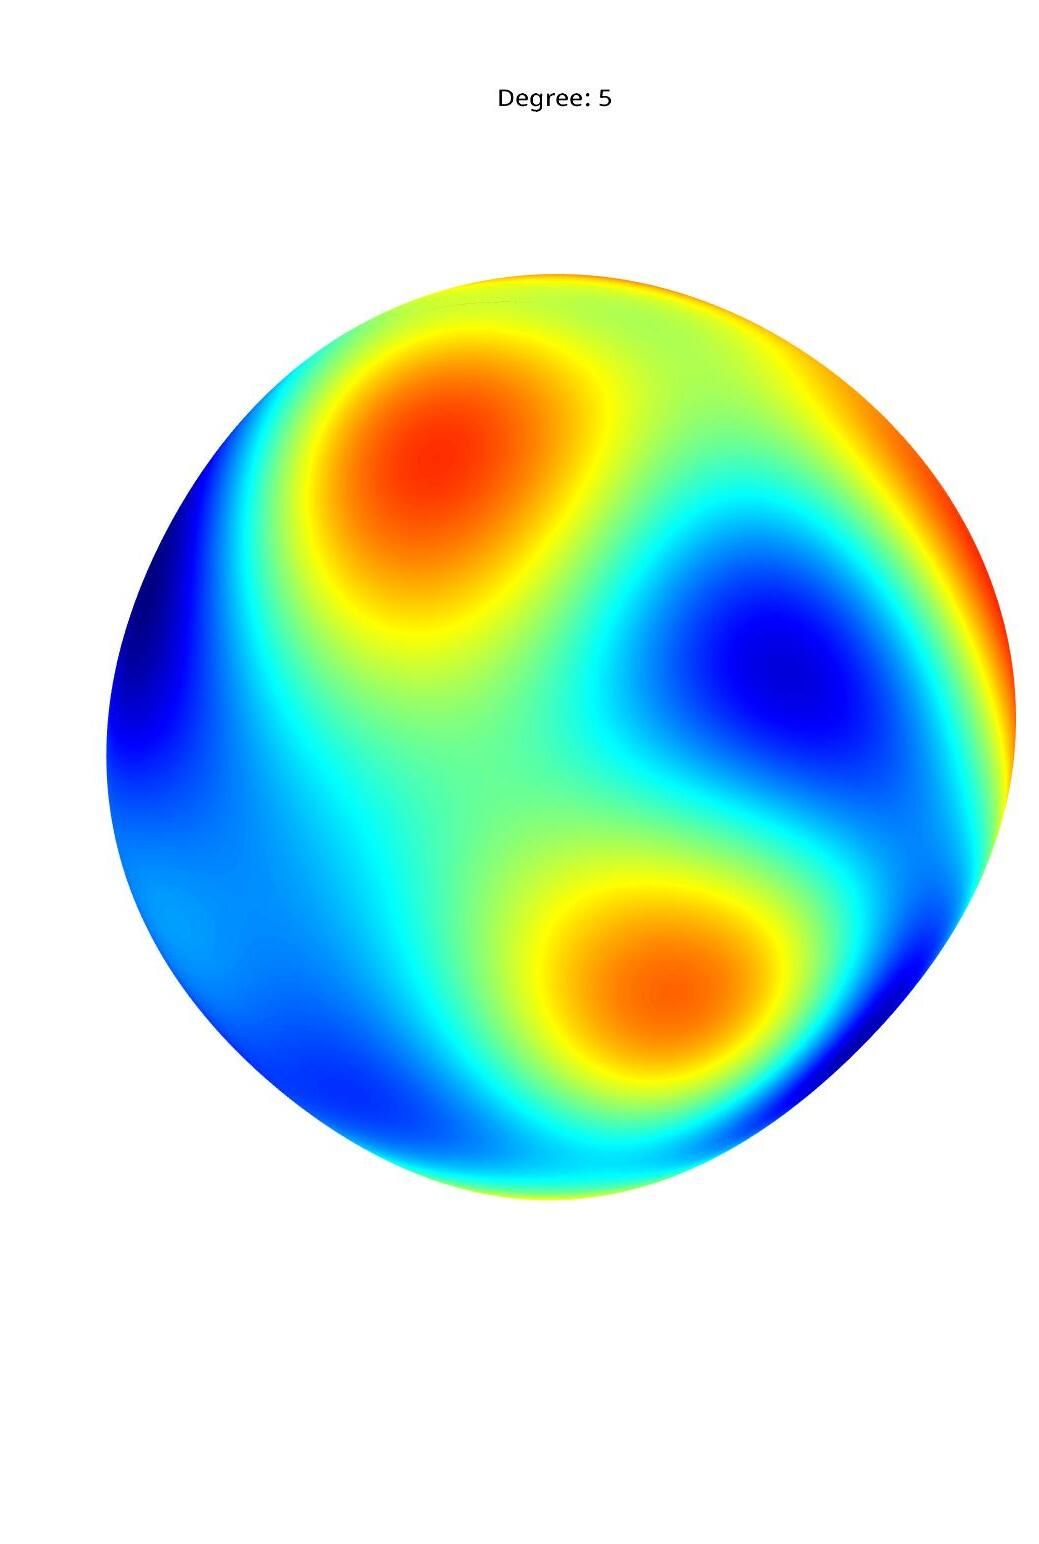
\includegraphics[width=0.95\linewidth]{media/med_5.jpg}
        \label{fig:med5}
    \end{minipage}
    \begin{minipage}{.245\textwidth}
        \centering
        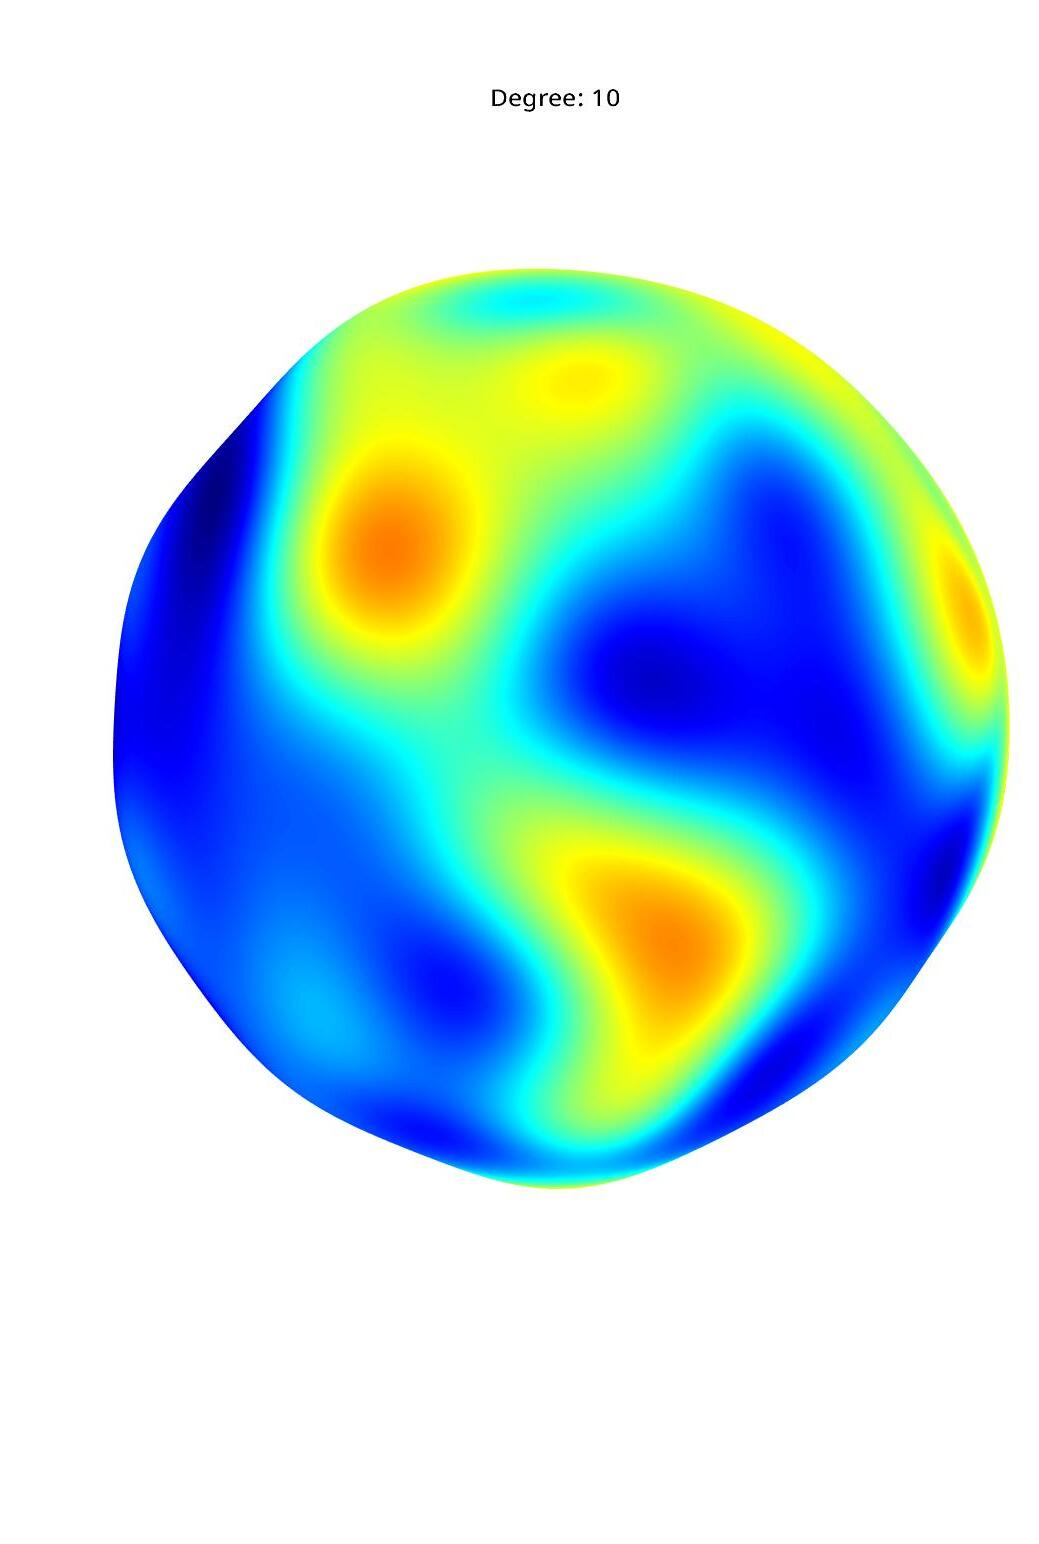
\includegraphics[width=0.95\linewidth]{media/med_10.jpg}
        \label{fig:med10}
    \end{minipage}
    \begin{minipage}{.245\textwidth}
        \centering
        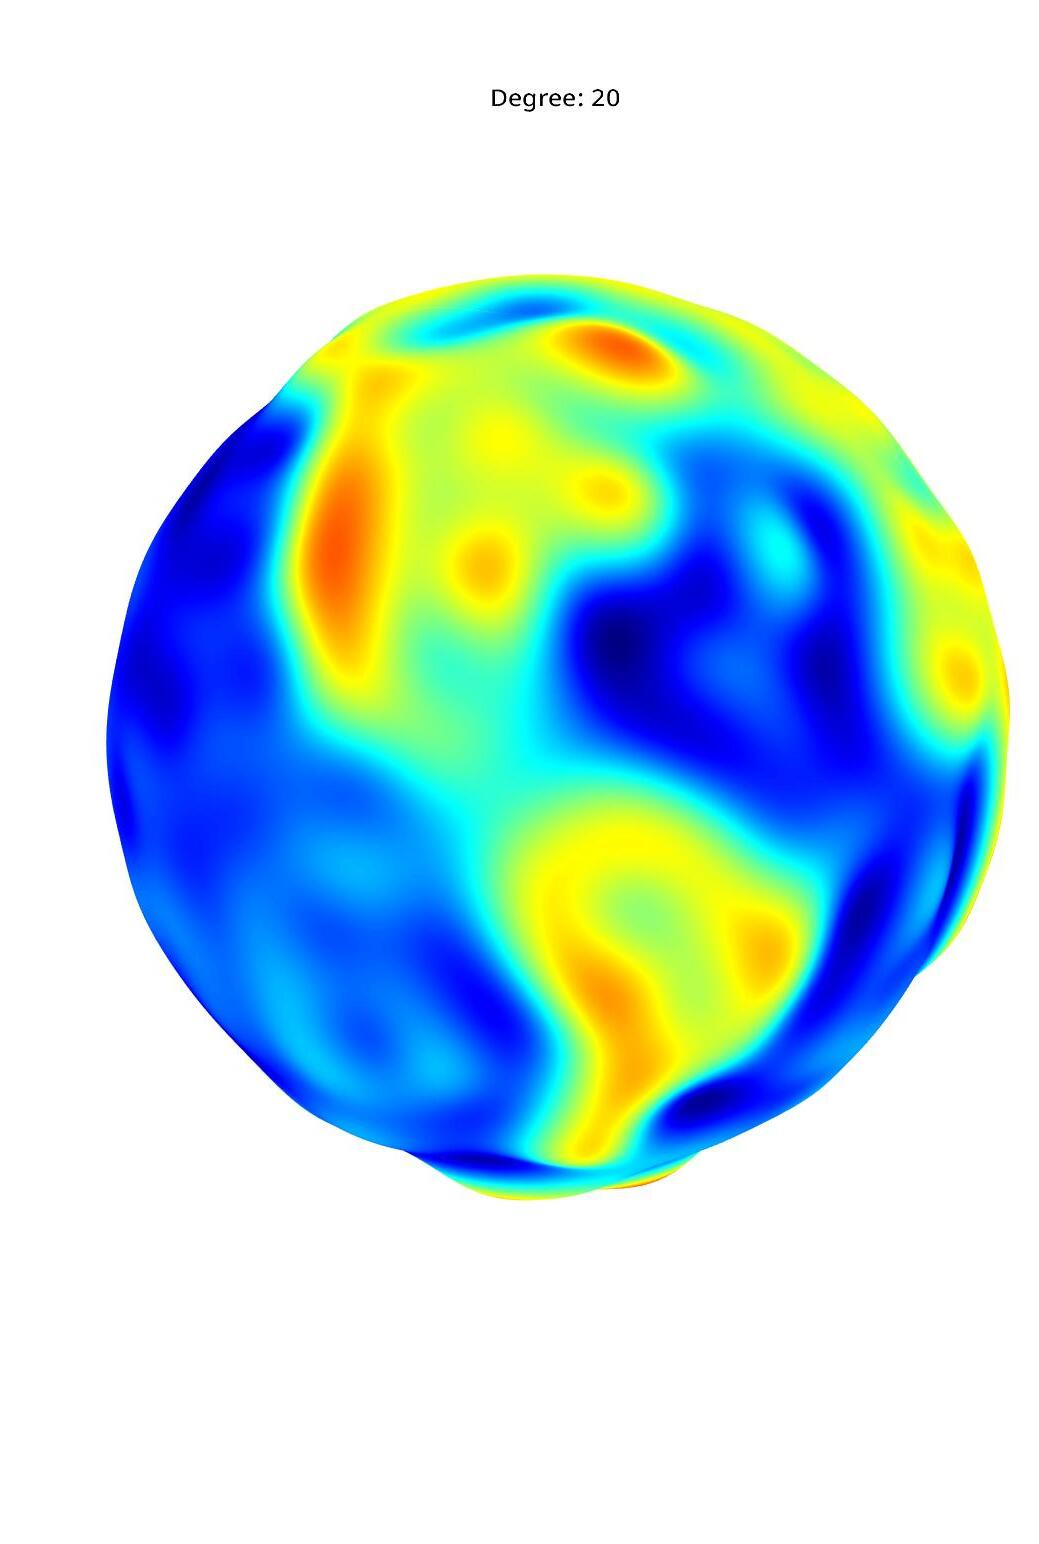
\includegraphics[width=0.95\linewidth]{media/med_20.jpg}
        \label{fig:med20}
    \end{minipage}
    \begin{minipage}{.245\textwidth}
        \centering
        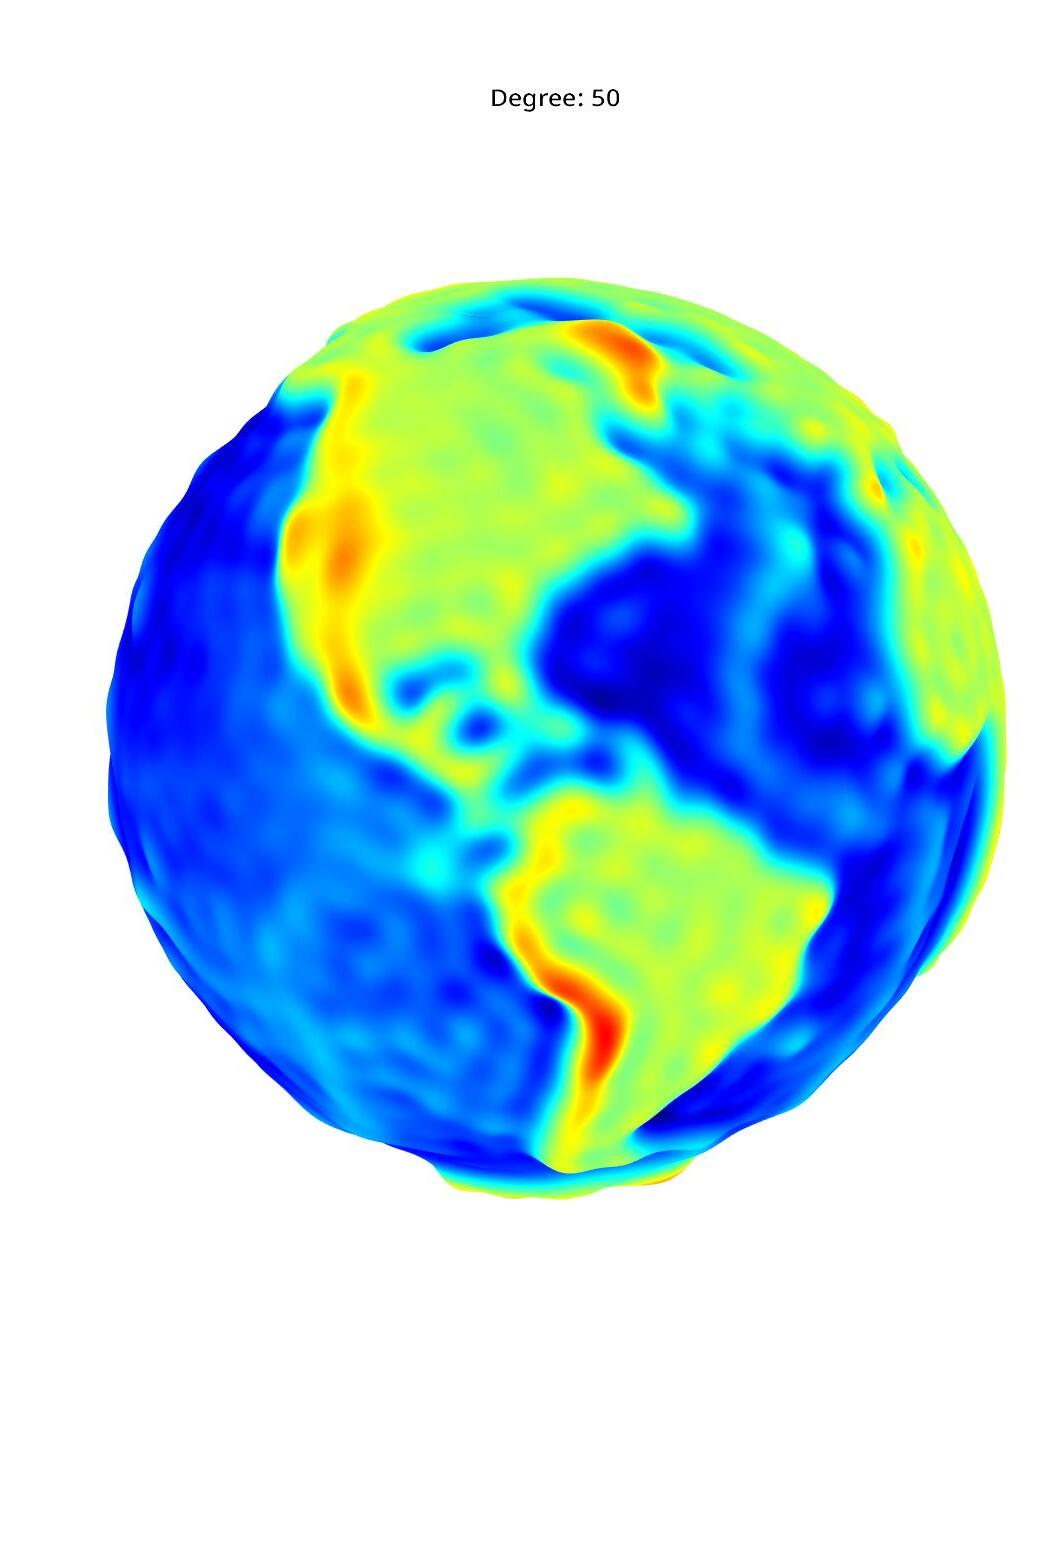
\includegraphics[width=0.95\linewidth]{media/med_50.jpg}
        \label{fig:med50}
    \end{minipage}
    \begin{minipage}{.245\textwidth}
        \centering
        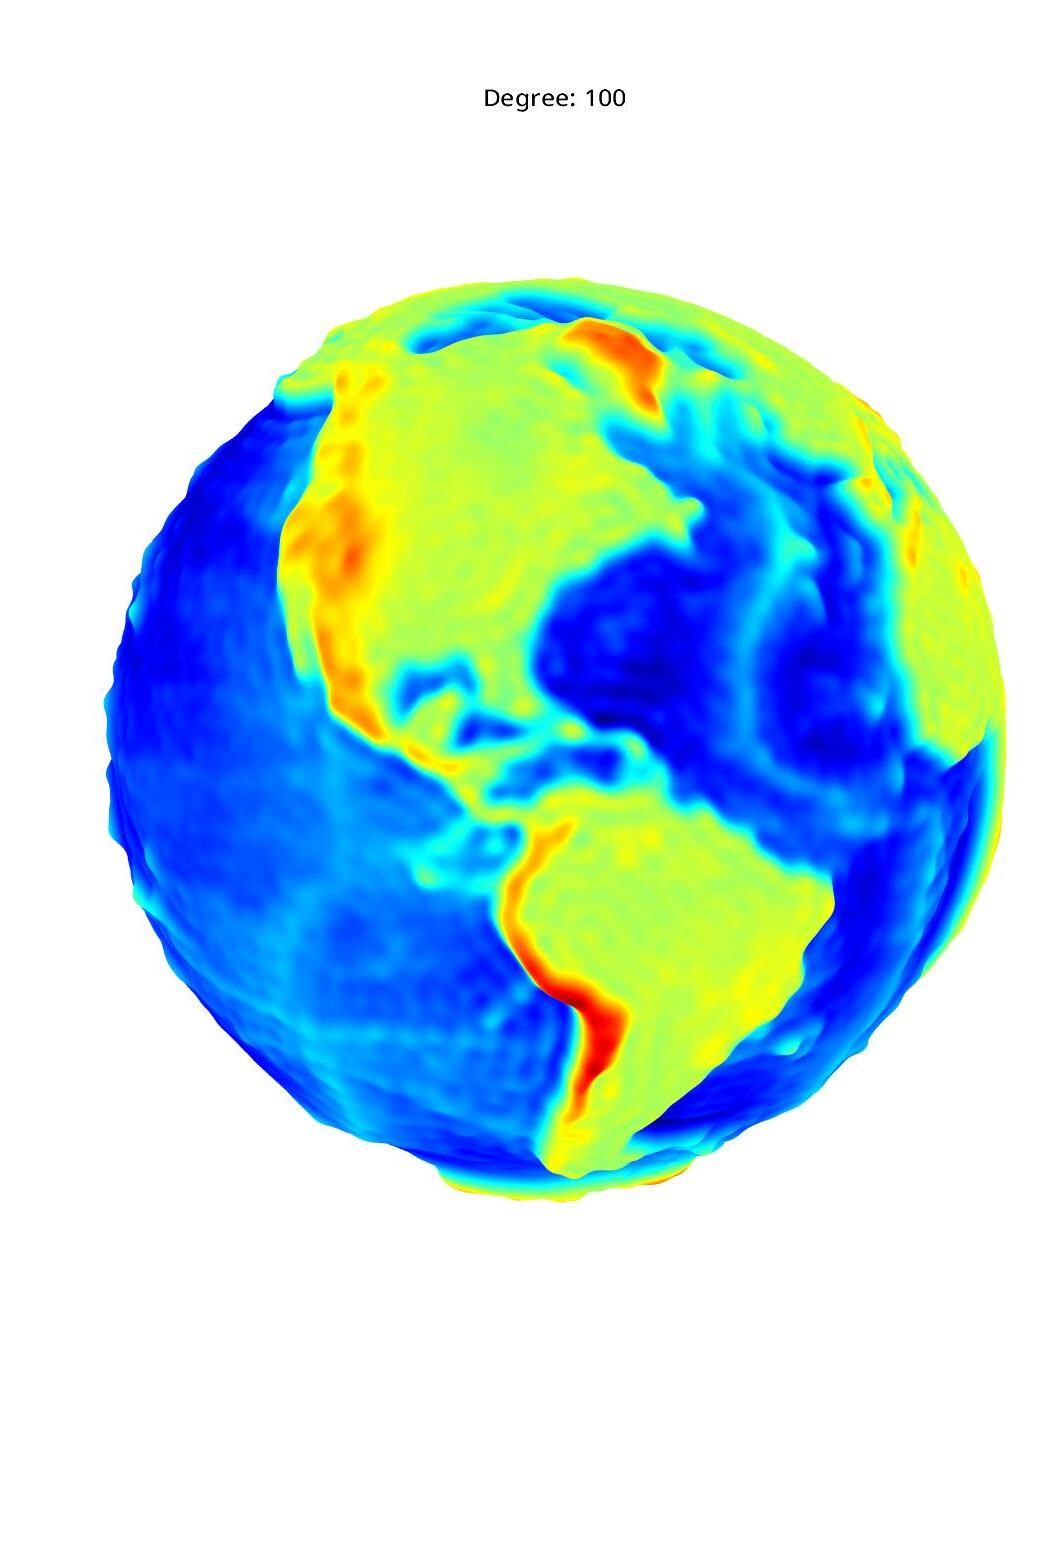
\includegraphics[width=0.95\linewidth]{media/med_100.jpg}
        \label{fig:med100}
    \end{minipage}
    \begin{minipage}{.245\textwidth}
        \centering
        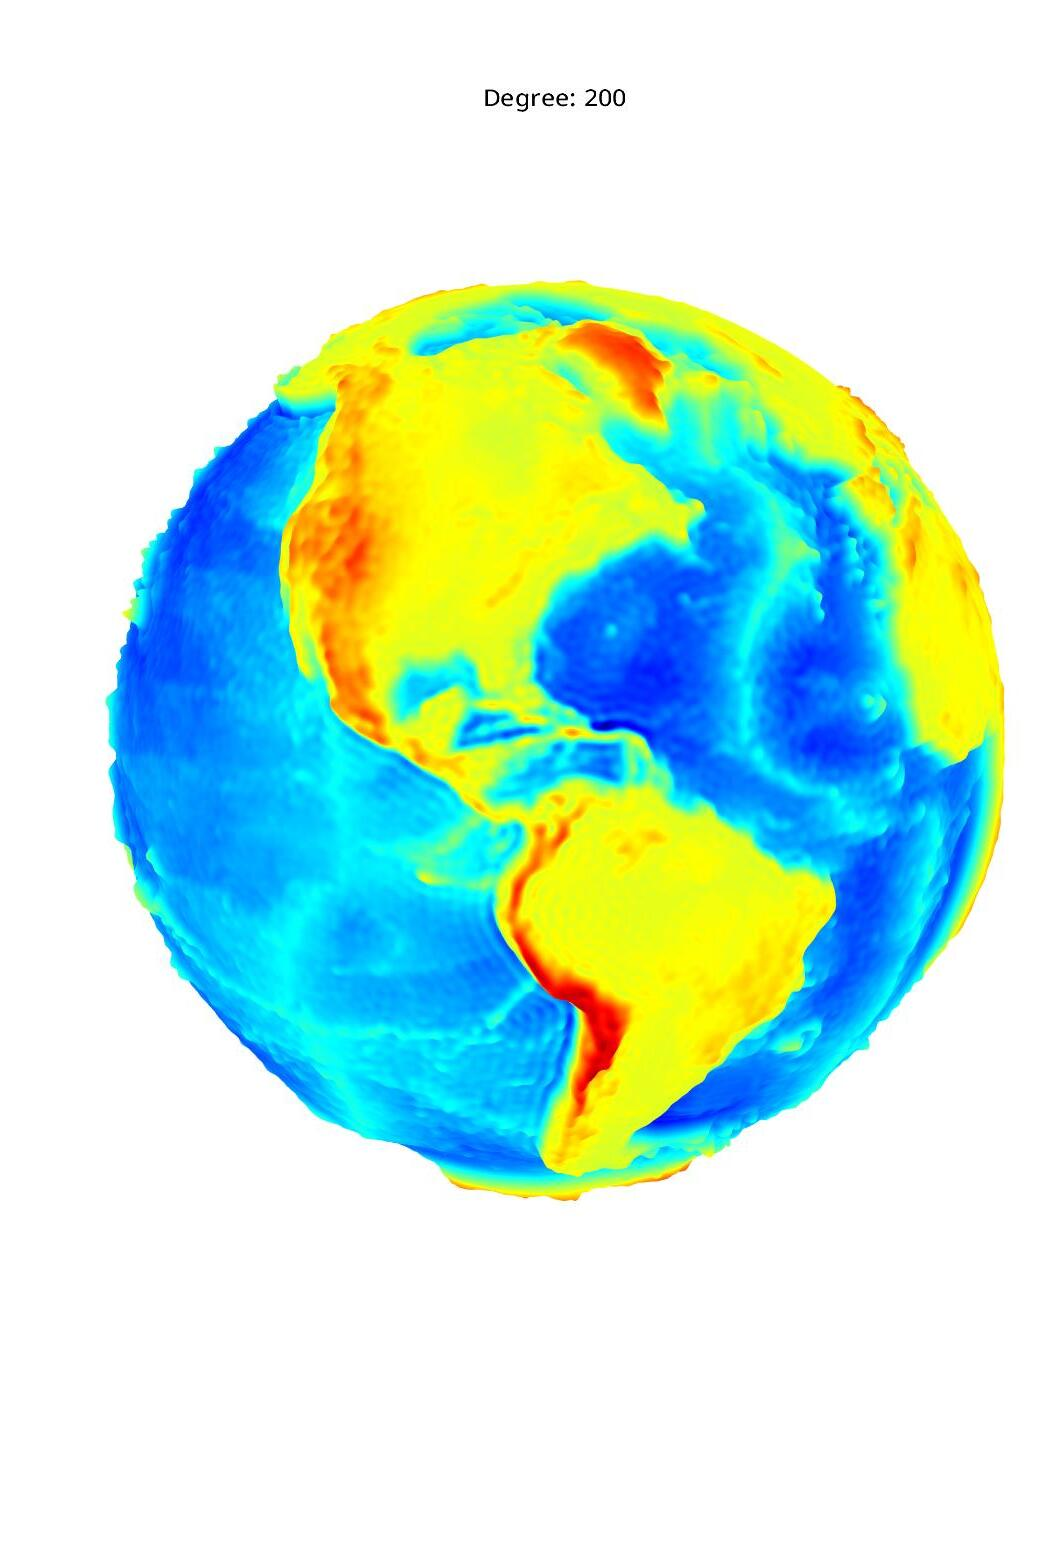
\includegraphics[width=0.95\linewidth]{media/med_200.jpg}
        \label{fig:med200}
    \end{minipage}
    \begin{minipage}{.245\textwidth}
        \centering
        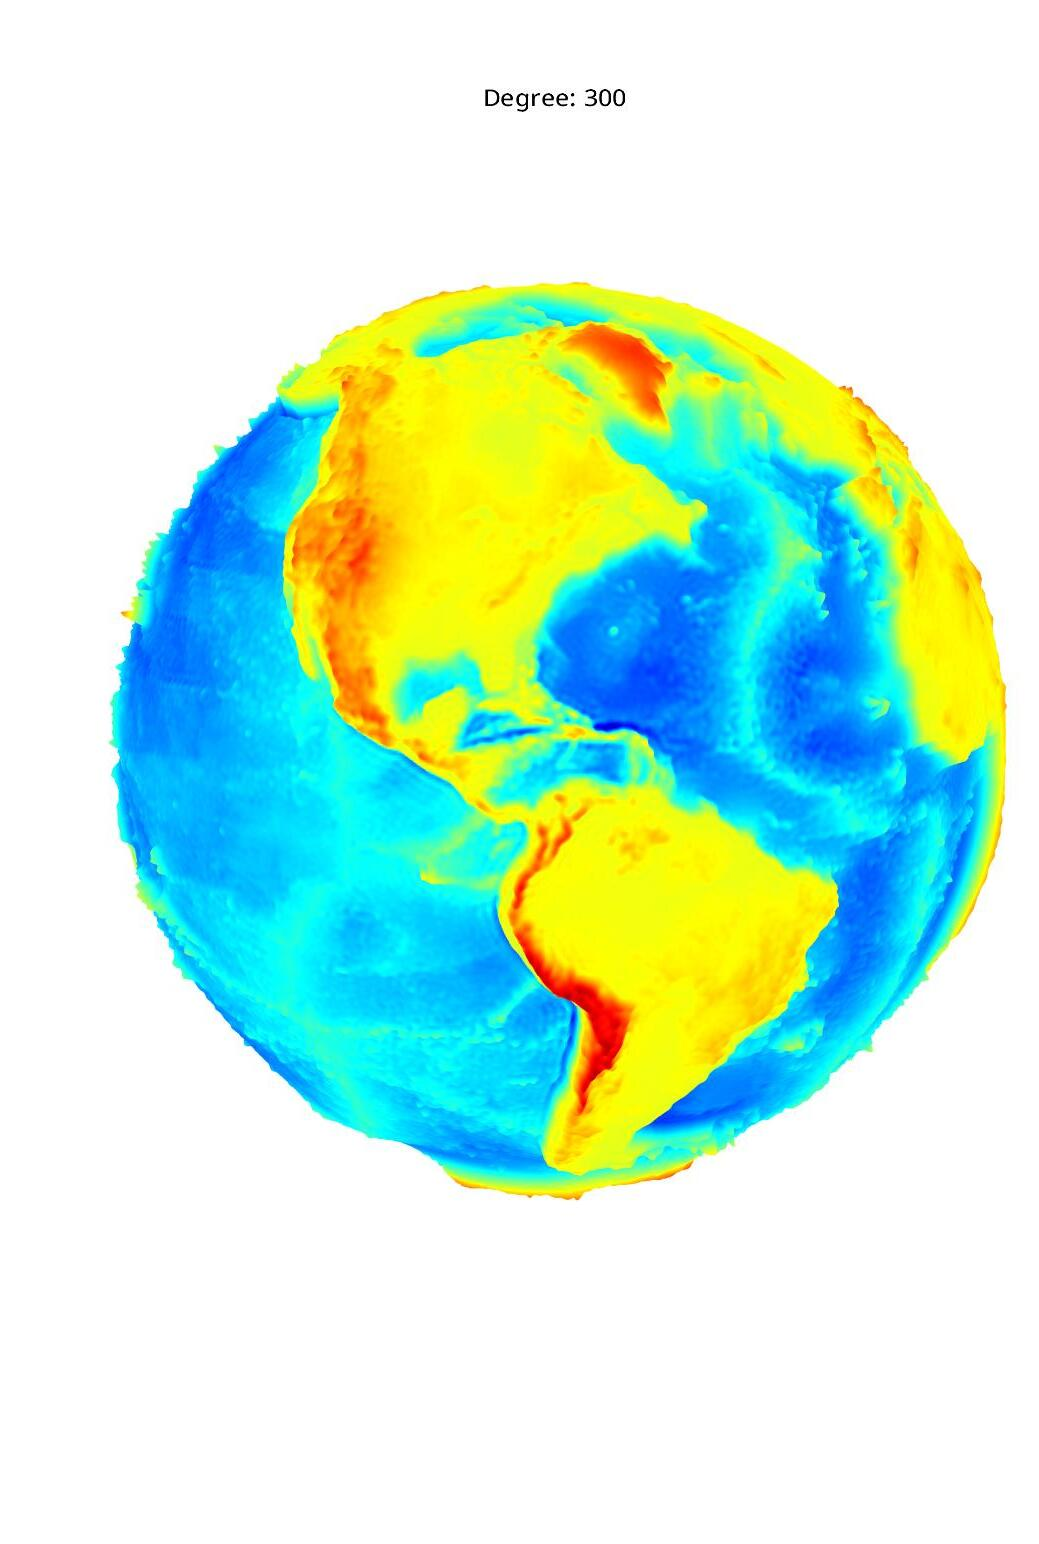
\includegraphics[width=0.95\linewidth]{media/med_300.jpg}
        \label{fig:med300}
    \end{minipage}
    \begin{minipage}{.245\textwidth}
        \centering
        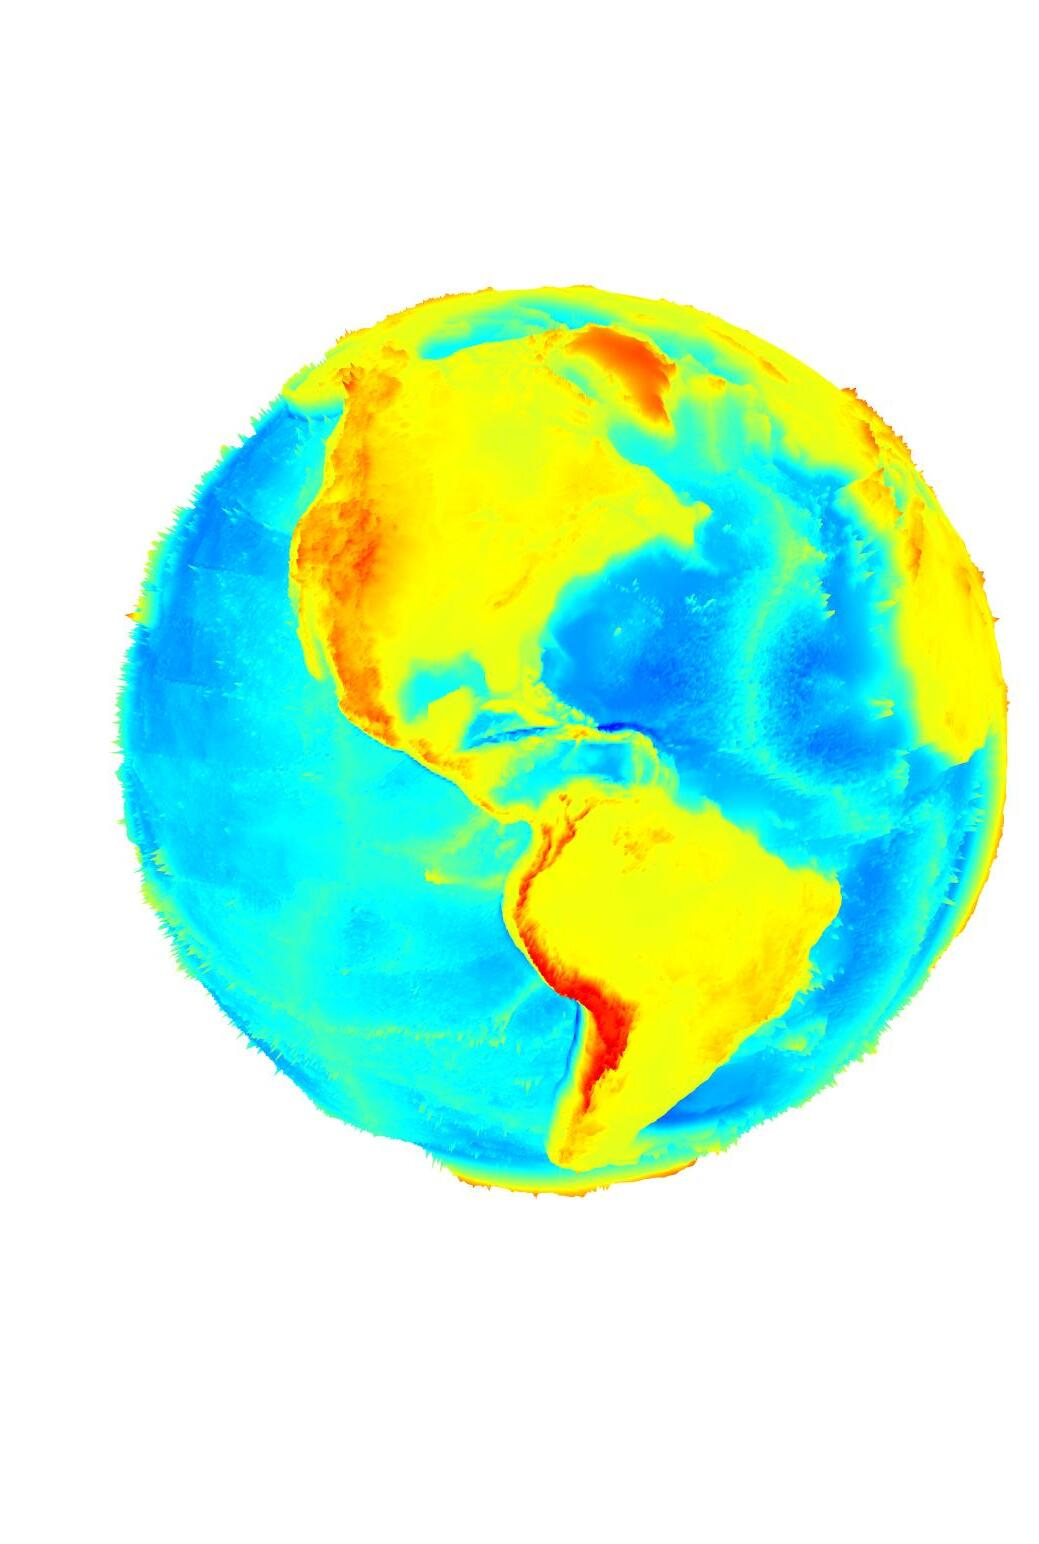
\includegraphics[width=0.95\linewidth]{media/med.jpg}
        \label{fig:med}
    \end{minipage}
    \caption{Altitude prediction of a model for varying degrees of a model. In the top row we have models of degree $l \in \{1, 2, 3, 4\}$, middle row $l \in \{5, 10, 20, 50\}$, and finally the bottom
    row $l \in \{100, 200, 300, +\infty\}$. The final visualization on the bottom right corresponds to the observed values of $f$.}
\end{figure}

Evidently, as we increase the degree of the model the difference between the predicted values $\hat f_i$ and the observations $f_i$ will tend to 
shrink in magnitude.

\begin{figure}
    \centering
    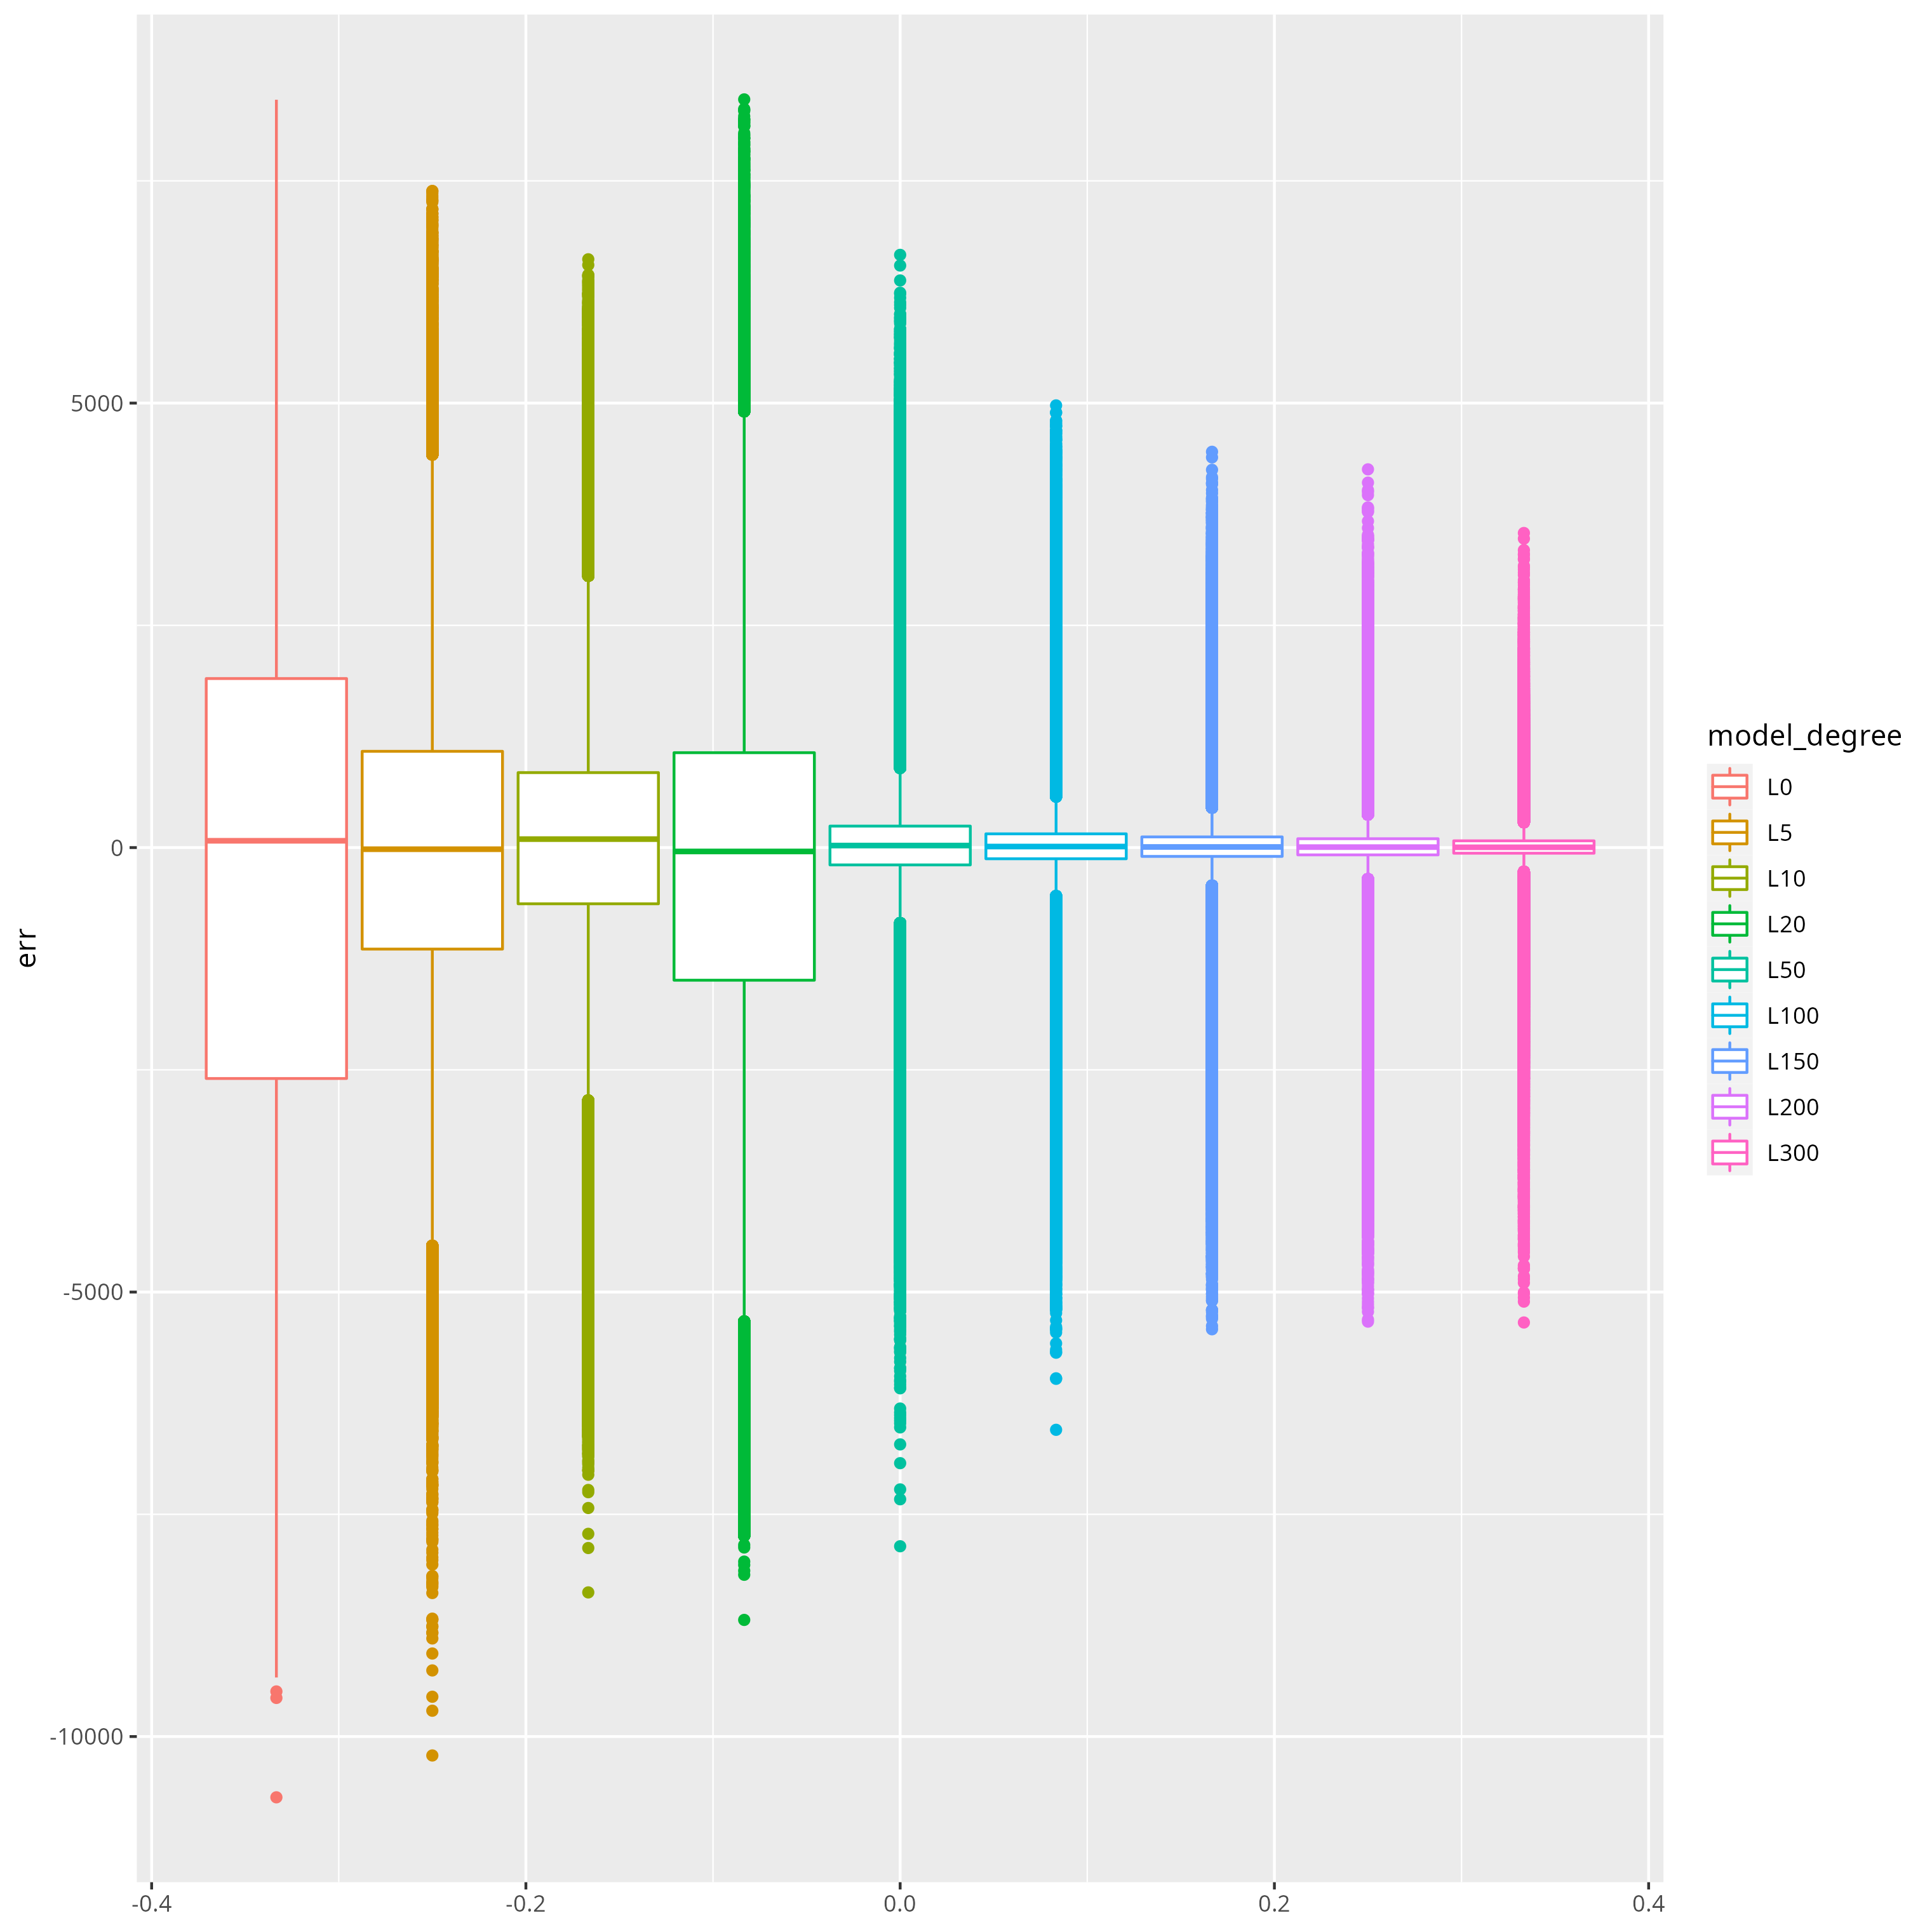
\includegraphics[width=0.5\linewidth]{media/boxplot_hi.png}
\end{figure}

\begin{figure}
    \centering
    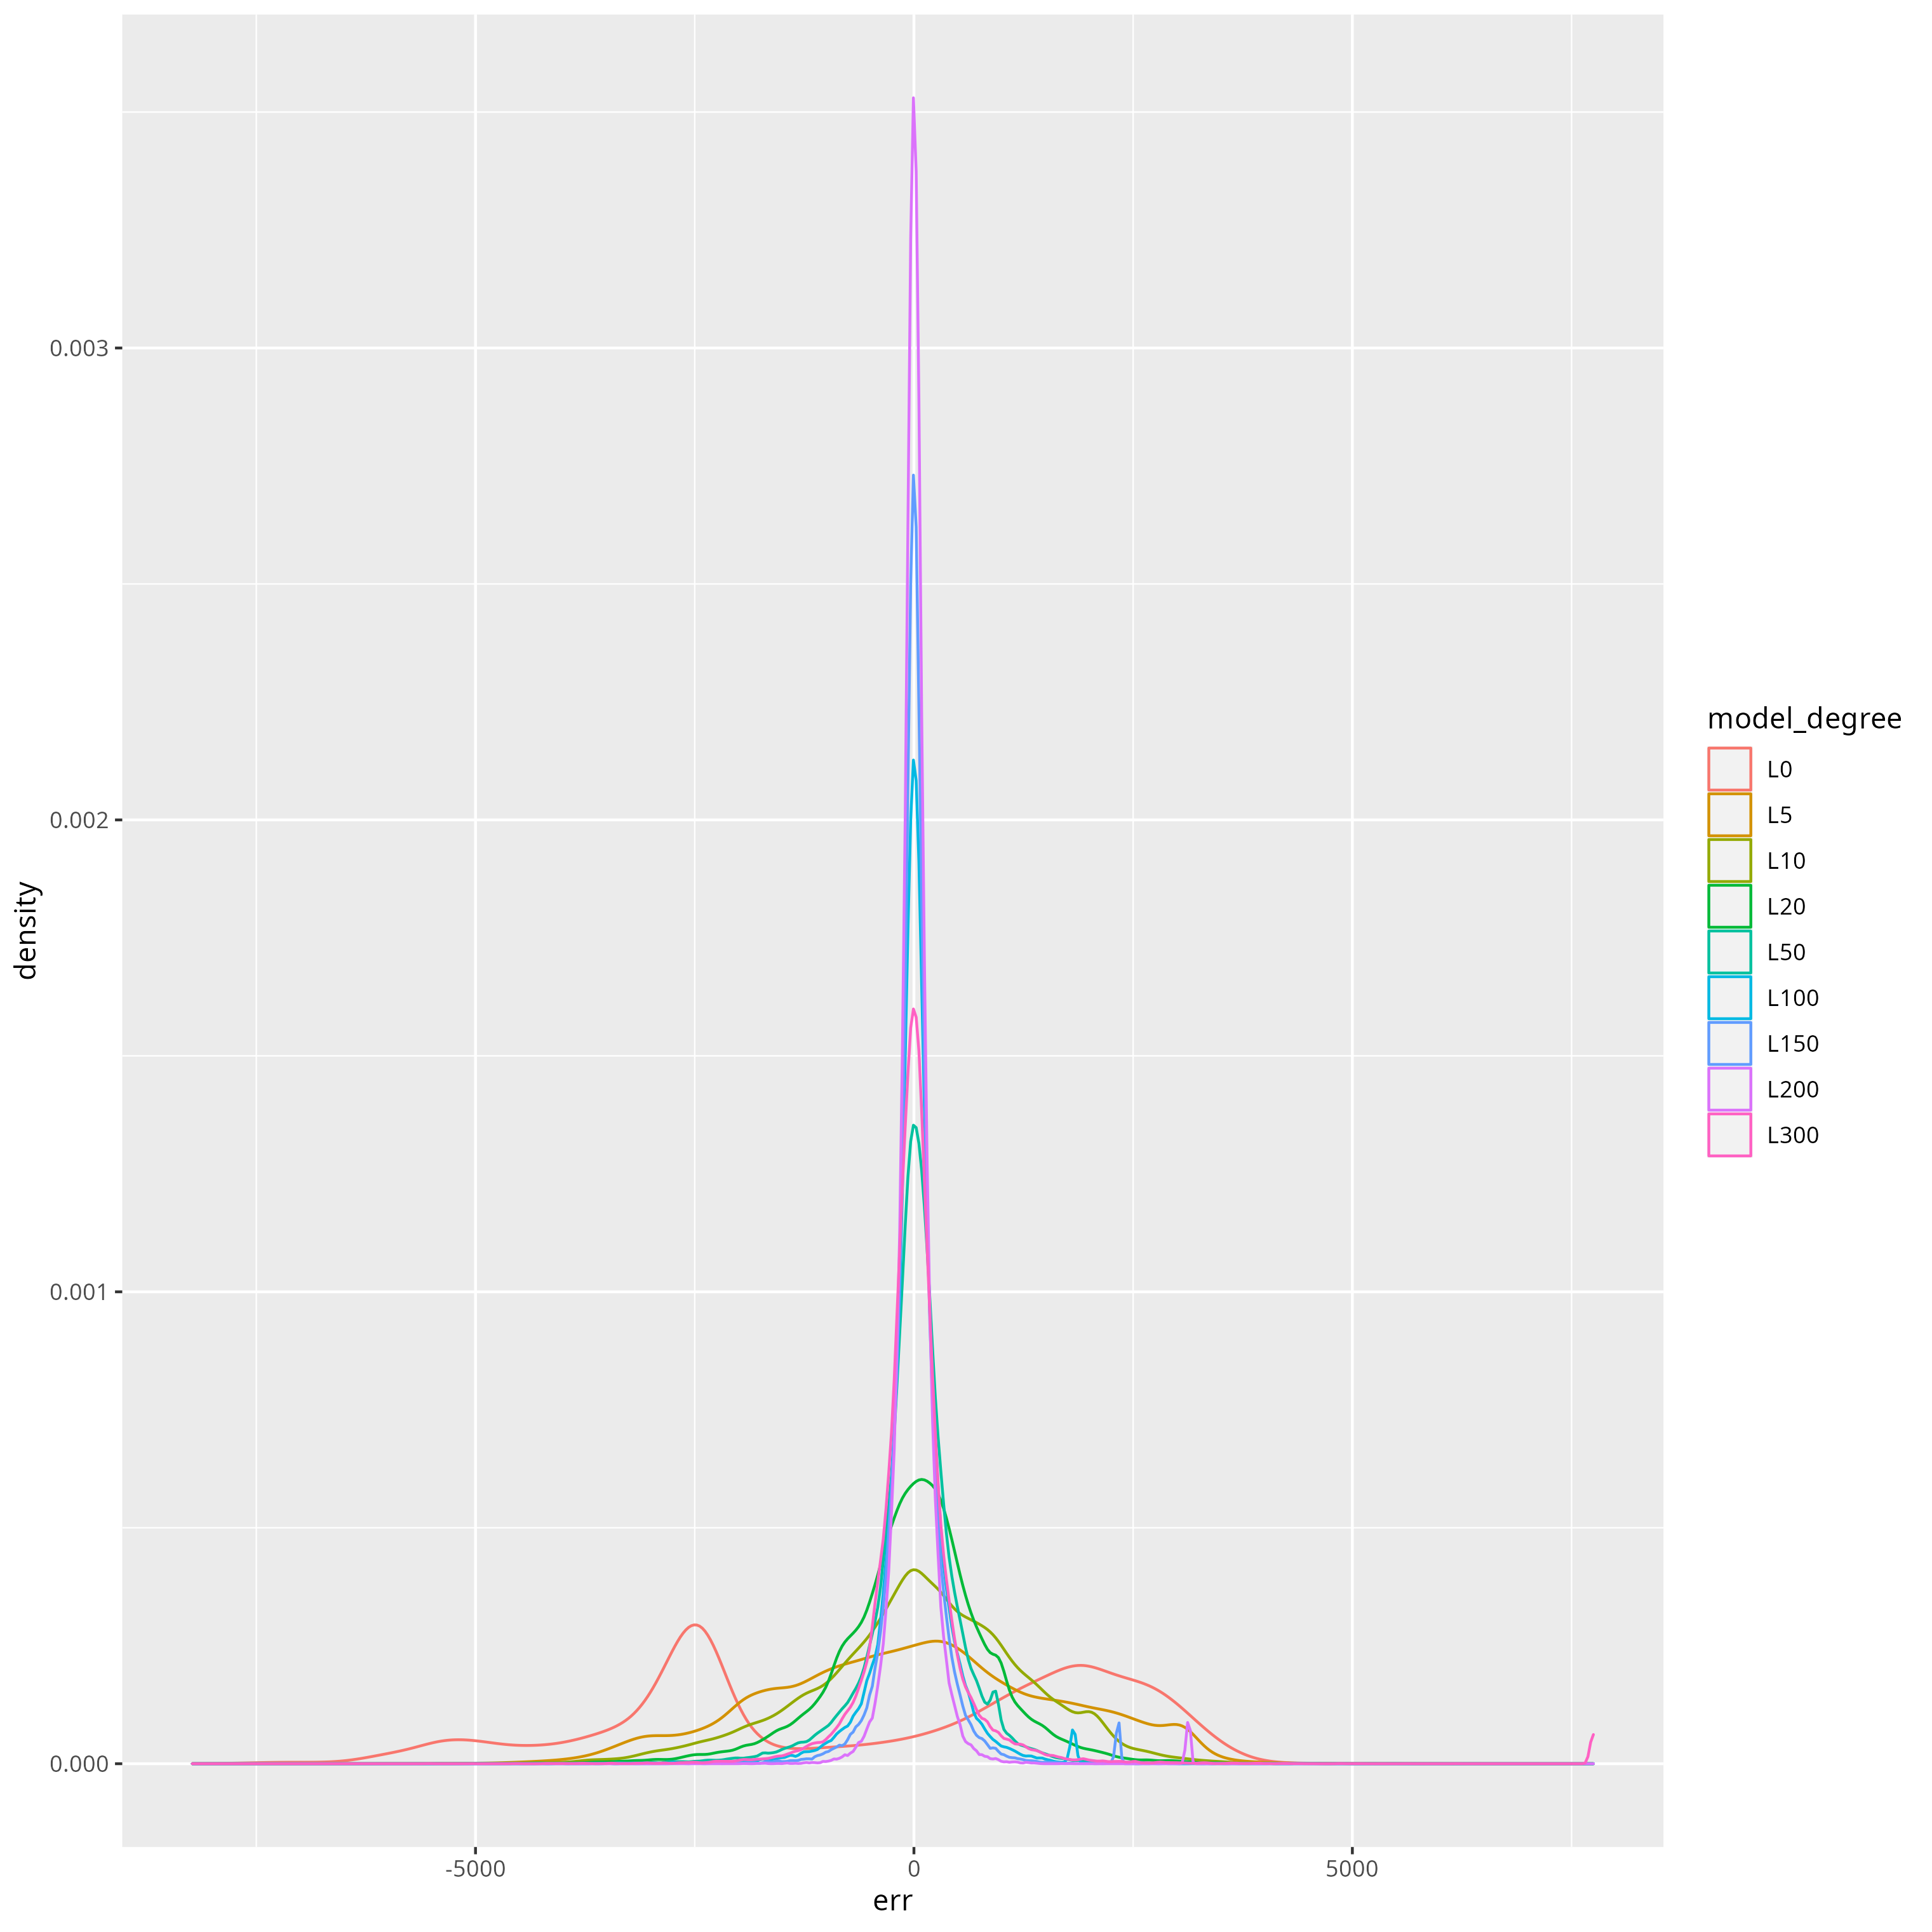
\includegraphics[width=0.5\linewidth]{media/density_small.png}
\end{figure}

\begin{figure}
    \centering
    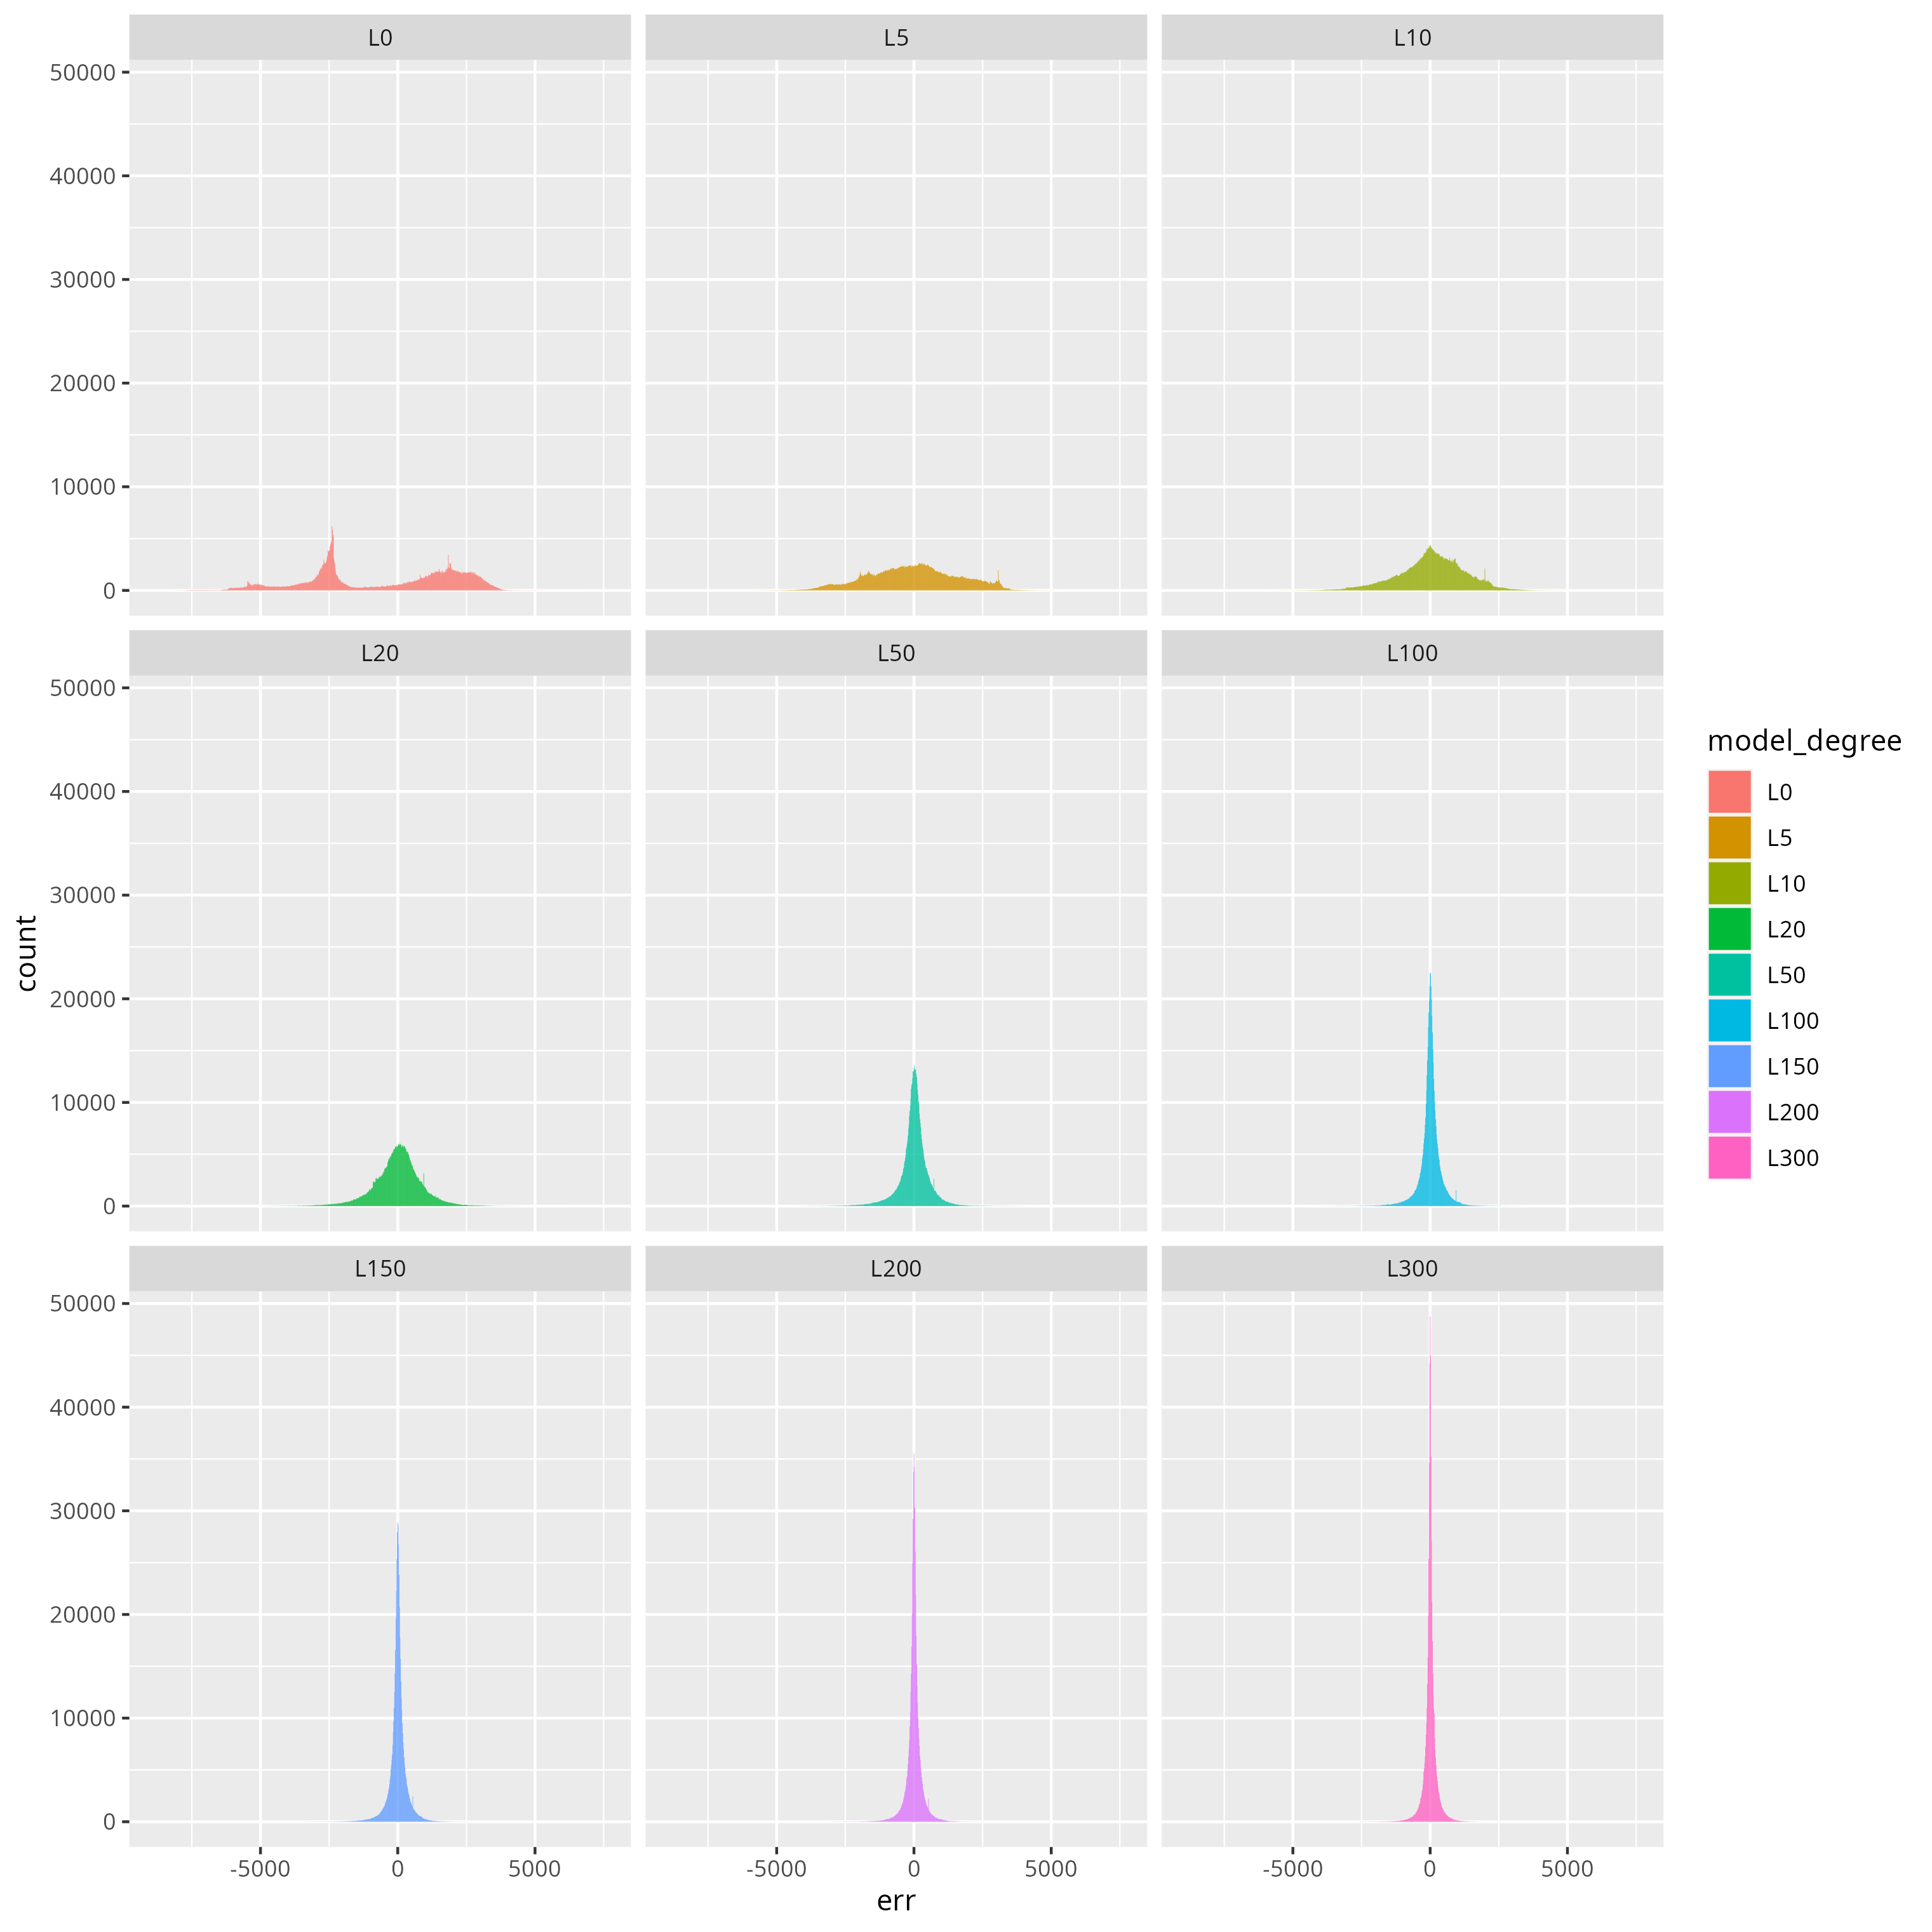
\includegraphics[width=0.5\linewidth]{media/faceted_histogram_med.png}

\end{figure}

\section{Parallelization} 

\textbf{TODO} (trivial)

\section{Conclusion}

Instead of calculating the model with a direct method that runs in $O(Nl_{max}^4)$ time, We propose a hybrid model that first directly computes the coefficients in $O(Nl_{max}^2)$ time then 
iteratively improves the MSE via stochastic methods running in $O(n_{training}n_{sample}l_{max}^2)$ time.

Results are to follow :)





\appendix
\section{Spherical Coordinates Transformation}

The data sets \verb|ETOPO1_*.csv| provided by NASA represent spherical coordinates in an unconventional format: $$(\phi, \lambda) \in [-\frac{\pi}{2}, \frac{\pi}{2}] \times [-\pi, \pi] $$ where $\phi$ refers to the latitude
and $\lambda$ refers to the longitude. In this section we outline the transformation from NASA's coordinate system to the ISO standard representation and prove equivalence between (1) and the Project presentation's $f(\phi, \lambda)$.

To avoid confusion, we denote the spherical coordinate pair in ISO coordinates as $(\theta_{iso}, \phi_{iso})$ and NASA's coordinate scheme as $(\phi_{nasa}, \lambda_{nasa})$.
We remark that the polar angle $\theta_{iso}$ is simply equal to $\frac{\pi}{2} - \phi_{nasa}$. We corroborate this fact by remarking that a latitude of $\phi_{nasa} = 0$ corresponds to a polar
angle of $\phi_{iso} = \frac{\pi}{2}$. Conveniently, the longitude $\lambda_{nasa}$ is equivalent to the azimuthal angle $\phi_{iso}$.

\begin{proposition} Let the spherial coordinate pairs $(\theta_{iso}, \phi_{iso})$, $(\phi_{nasa}, \lambda_{nasa})$ be defined as above. 
    \begin{equation*}
        f(\theta_{iso}, \phi_{iso}) \equiv f(\phi_{nasa}, \lambda_{nasa})
    \end{equation*}

    
\end{proposition}



\begin{proof}
    $f(\phi_{nasa}, \lambda_{nasa})$ is defined in the Project proposal as 
    \begin{align} \label{eq:project_def} 
        f(\phi_{nasa}, \lambda_{nasa}) &= \sum_{l = 0}^{+\infty}\sum_{m = 0}^l \bar P_l^m(\sin\phi_{nasa})[C_l^m\cos m\lambda_{nasa} + S_l^m \sin m \lambda_{nasa}] \\ 
                                       &= \sum_{l = 0}^{+\infty}\sum_{m = 0}^l \bar P_l^m(\sin(\pi/2 - \theta_{iso}))[C_l^m\cos m\phi_{iso} + S_l^m \sin m \phi_{iso}] \\
                                       &= \sum_{l = 0}^{+\infty}\sum_{m = 0}^l \bar P_l^m(\cos\theta_{iso}))[C_l^m\cos m\phi_{iso} + S_l^m \sin m \phi_{iso}] \\
                                       &\equiv f(\theta_{iso}, \phi_{iso})
    \end{align}

\end{proof}

\nocite{*}

\bibliography{ppar}
\bibliographystyle{ieeetr}

\end{document}

